\chapter{Computer Architecture}

\newpage

\section{ISA1}
%\noindent\textbf{MIPS instructions} \newline
\subsection{MIPS instructions}
The instructions that a assembly languge use for the MIPS proses.
% https://www.dsi.unive.it/~gasparetto/materials/MIPS_Instruction_Set.pdf

\noindent\textbf{Terminology} \newline
\begin{itemize}
\item  Register file: 32 registers from R0-R31, each is 32 bits.
\item  Memory: Large each adders stores a word (4 x Registers). Address is all ways increments of 4.
       Memory is segmented into 4 8-bits of data to create a word.
\item  PC (Project counter): Increase with 4 each time to go to the next memory address.
\item  Instruction Registers: Retrieve the current instructions.
\item  Control: Inserts data to the register file and add the operation to ALU (Compute).
\item  ALU (Compute): Calculates the value.
\item  Memory Address: Call the value from a specific address. From ex ``lw''.
\item  Data Register: Retries and directs value from memory to register file.
\end{itemize}

\newpage
\emph{note:} memory operations like (sw R1, 0(R2)) stores the word in poison R2+0 where 0 is the increment
since if it is a loop it is needed. The value at that position is R1. 

\noindent\textbf{The operations most used} \newline
\begin{figure}[h]
    \vspace{10mm}
    \centering
    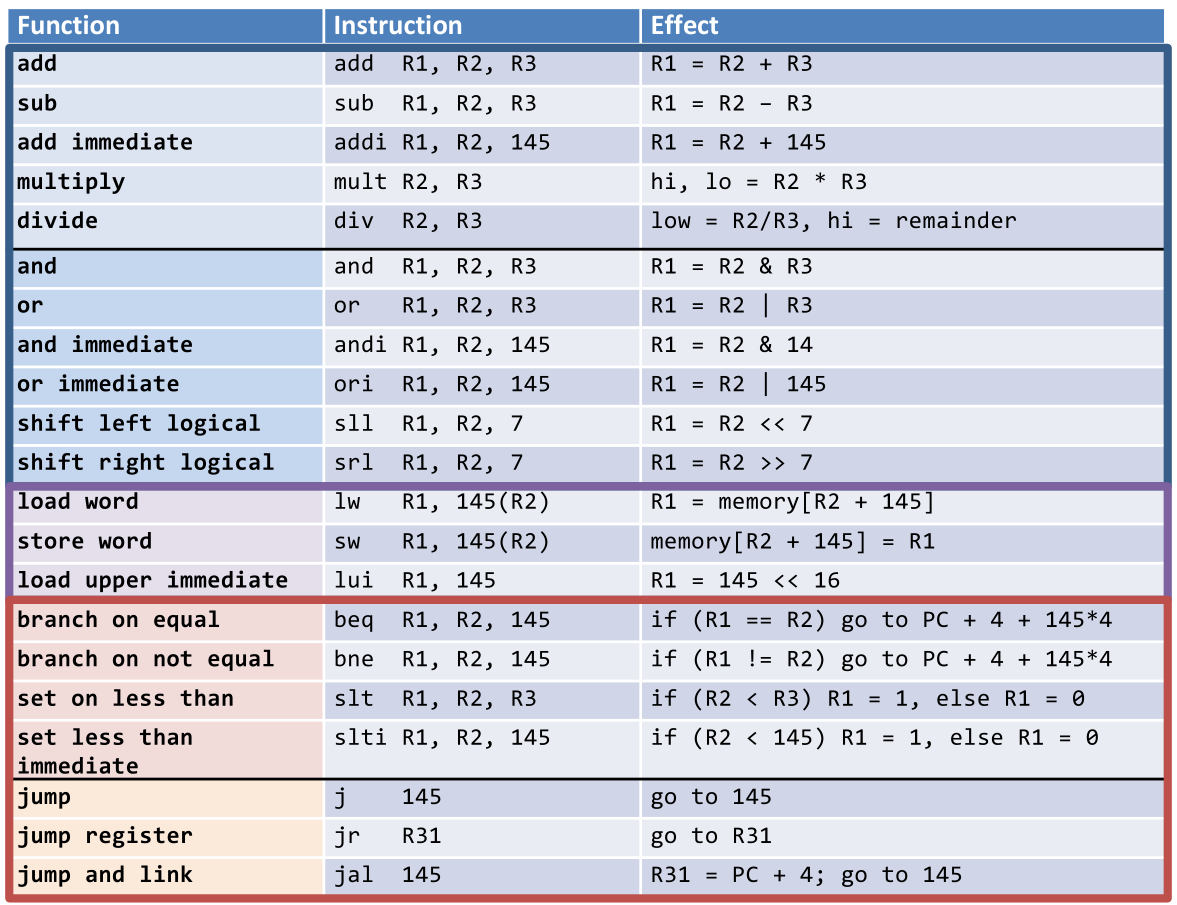
\includegraphics[width=16cm, height=13cm]{image/mips-tabel.png} 
    \caption{MIPS oporation tabel}
\end{figure}

\newpage

\subsection{Sequencing}
\begin{figure}[h]
    \vspace{10mm}
    \centering
    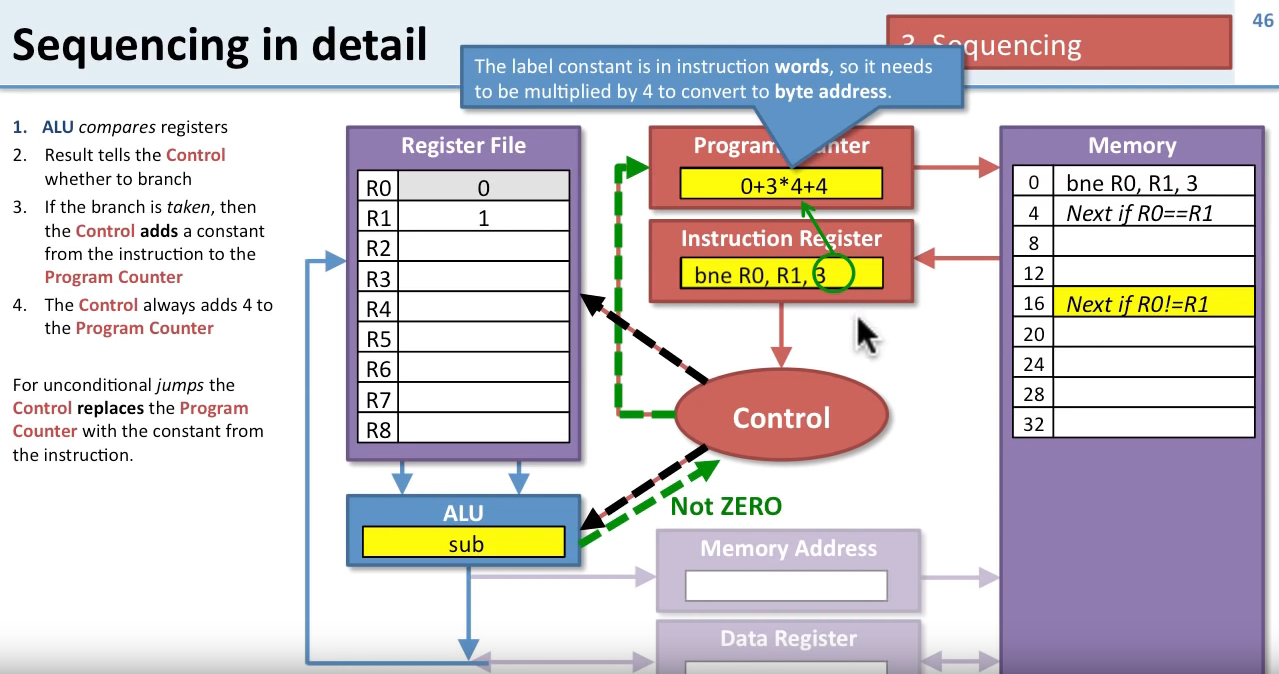
\includegraphics[width=16cm, height=10cm]{image/sequencing.png} 
    \caption{Sequencing}
\end{figure}
\newpage

\subsection{Converge to Assambly code}
\noindent\textbf{If Else example} \newline
\begin{figure}[h]
    \vspace{10mm}
    \centering
    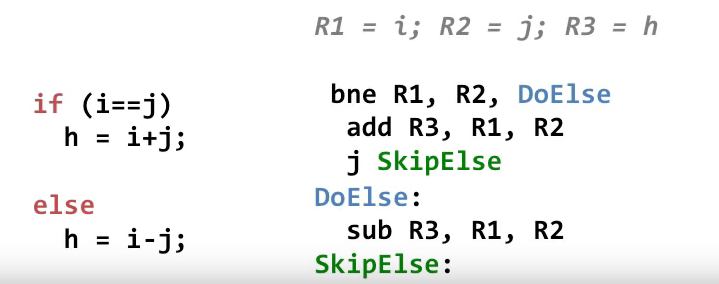
\includegraphics[width=10cm, height=5cm]{image/assambly-exampel.png} 
    \caption{Assambly exampel}
\end{figure}

\section{ISA2}
%https://inst.eecs.berkeley.edu/~cs61c/resources/MIPS_help.html
\subsection{MIPS type format}
\begin{itemize}
\item  R-format, Aretmetic and lodgical \newline
  op: ex add \newline
  rs: first register \newline
  rt: second register \newline
  rd: destination register \newline
  shmt: shift amount \newline
  funct: Function selector (add = 32, sub =34)
\item  I-format, Load/store, branch and intemidiats \newline 
  op: ex addi, beq \newline
  rs: first register \newline
  rt: second register \newline
  rd: inttediate value 
\item  J-format, Jump 
  op: ex j skipelse \newline
  rd: address   
\end{itemize}

\begin{figure}[h]
    \vspace{10mm}
    \centering
    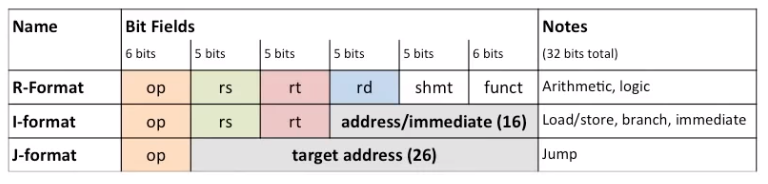
\includegraphics[width=17cm, height=6cm]{image/mips-types.png} 
    \caption{MIPS Types}
\end{figure}

A instruction allwas ends with 00 it means that when a instruction is done we update the program couner
to by 4 or more it changes the posistion of the 16bit intermidjet for i-format and can. (bne, beq)

\subsection{Procedure}
Procedure is how a function call is handeld. It is devided into two parts Caller and Callee,
the caller call the procedure (callee).
The oporation for contolling procedure is called jump-and-link (jal).
It stores the return address (PC+4) in \$ra (R31).
Where (ra = register address (updates automatically))
(PC = project counter)
(R31 = value).
jr \$ra returns the value.

\subsubsection{Stacking}
To avoid conflicts with writing over the callers register files, one uses staking in predefined
ranges to allow store data independent from the callers. 
(R29 =  store stack data \$sp)
When a register file is added the stock pointer is moved and when it is done it returns with (jr) and then
reset the previously used register files.
when it has used what it needs it removes them when leaded one value at a time


\begin{figure}[h]
    \vspace{10mm}
    \centering
    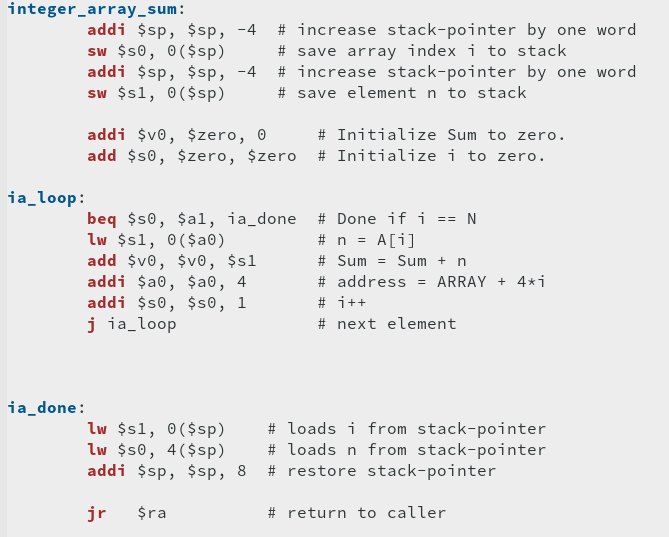
\includegraphics[width=16cm, height=12cm]{image/code-ex.png} 
    \caption{code ex}
\end{figure}

\begin{figure}[h]
    \vspace{10mm}
    \centering
    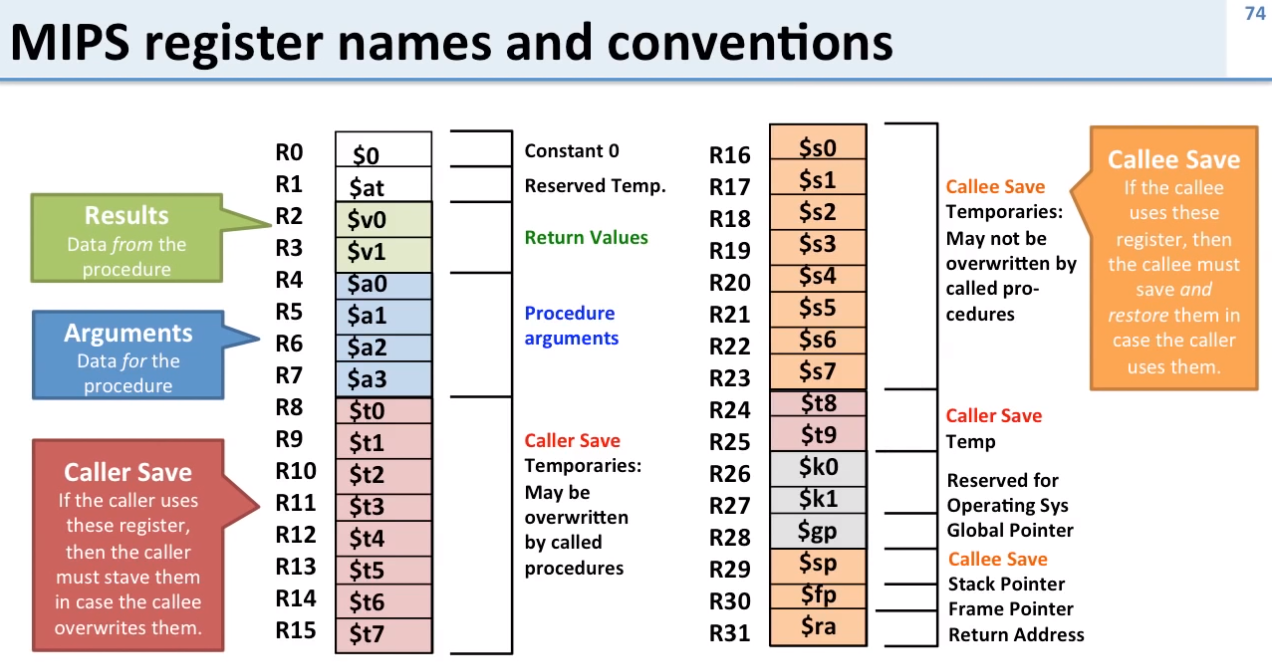
\includegraphics[width=16cm, height=8cm]{image/mips-register.png} 
    \caption{MIPS register}
\end{figure}

Notice that the register files for the callee save is \$sx and for the caller \$tx.

\newpage
\subsection{Other ISA}
\begin{figure}[h]
    \vspace{10mm}
    \centering
    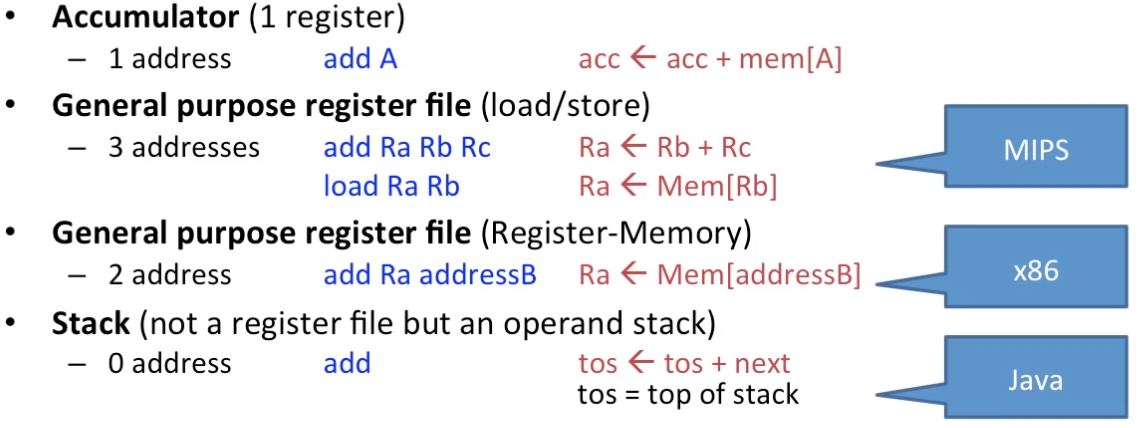
\includegraphics[width=16cm, height=6cm]{image/other-isa.png} 
    \caption{Other ISA}
\end{figure}

\begin{figure}[h]
    \vspace{10mm}
    \centering
    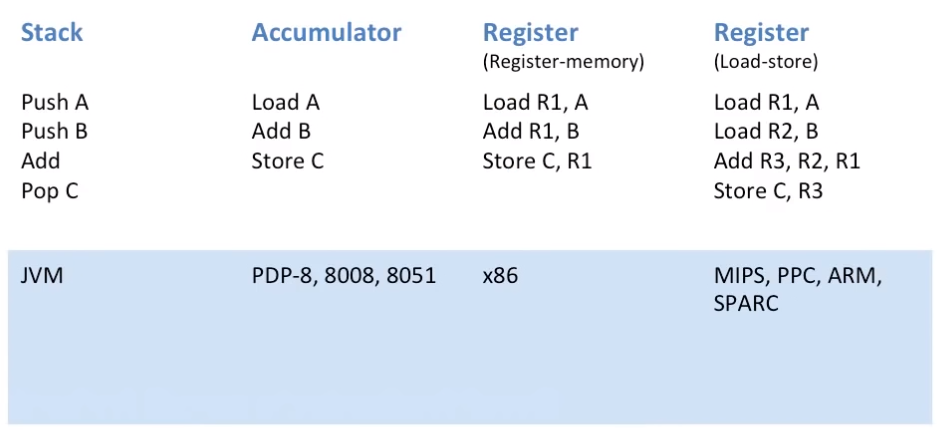
\includegraphics[width=16cm, height=6cm]{image/other-isa-instructions.png} 
    \caption{Other ISA instructions}
    \label{other-isa-instructions}
\end{figure}



\newpage


\section{Arithetic}

\subsection{Binary numbers}
\begin{itemize}
\item  Binary numbers reduses noice and disregard the exact voltitge to rusult in on off mode.
\item  In comuter sience octal and hexadecimals are also often used becose of it properties.
  every octo didgets represent 3 in decimal
  every hex didgets represent 4 in decimal
\item  msb=most significant bit
\item  lsb=lest significant bit
\item  Optemazation: $0010*0101$  2 oporations $\to 0101*0010$  1 oporations
\item  Multiplication: (fixed point need to shift desimal point)
  $0010 * 0101 = 0010 + (0010 shifting[00]) = 1010$
  $0011.010 * 0001.110 = $
\item  Addition: (Same for fixed points and integers)
  $1110+1000= carry[1] 0110$ Overflow
  $0101+0001= 0110$ Not overflow
\end{itemize}

\subsection{Negative integes}
\begin{itemize}
\item  \emph{Signed magnetude:} msb is the sign
  ${1011}_2 = {-(2+1)}_{10} = {-3}_{10}$
\item  \emph{tow's complement:} if msb is 1 then negative number every other digiet after is positiv
  ${1011}_2 = {-8 +2 +1}_{10} = {-5}_{10}$
\end{itemize}


\subsection{Oporations}

\subsection{Non integer numbers (Floating and fixed point)}
\begin{itemize}
\item  Converting binary to decimal:
  $0.111 = 1/2 + 1/4 + 1/8= 0.875$
\item  Fixed point: for defined ranges $1.001$ and $0.100$ one can chose large and small representations
\item  Floating point:  IEEE standard, se following image
\item  Standard floting point is in binary so FFFF is at most 1111 and with two's complement  0111
\end{itemize}

\begin{figure}[h]
    \vspace{10mm}
    \centering
    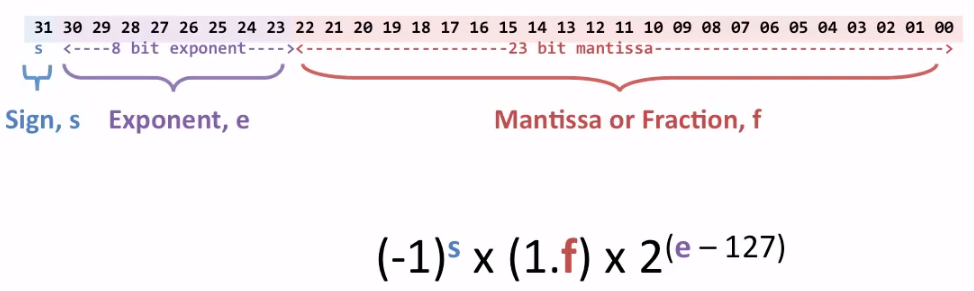
\includegraphics[width=16cm, height=5cm]{image/floating-point.png} 
    \caption{Floating Point}
    \label{floating-point}
\end{figure}

\subsection{Overflow}
\begin{itemize}
\item  input: msb = 1 for boath numbers and output: msb = 0 (overflow)
\item  input: msb = 0 for boath numbers and output: msb = 1 (overflow)
\item  input: msb = 0 for boath numbers and output: msb = 0 (Not overflow)
\item  input: msb = 1 for boath numbers and output: msb = 1 (Not overflow)
\item  input: msb = 1 and msb = 0 (Maby overflow)
\end{itemize}


\newpage

\section{Logic}
% https://aur.archlinux.org/packages/logisim/

\begin{figure}[h]
    \vspace{10mm}
    \centering
    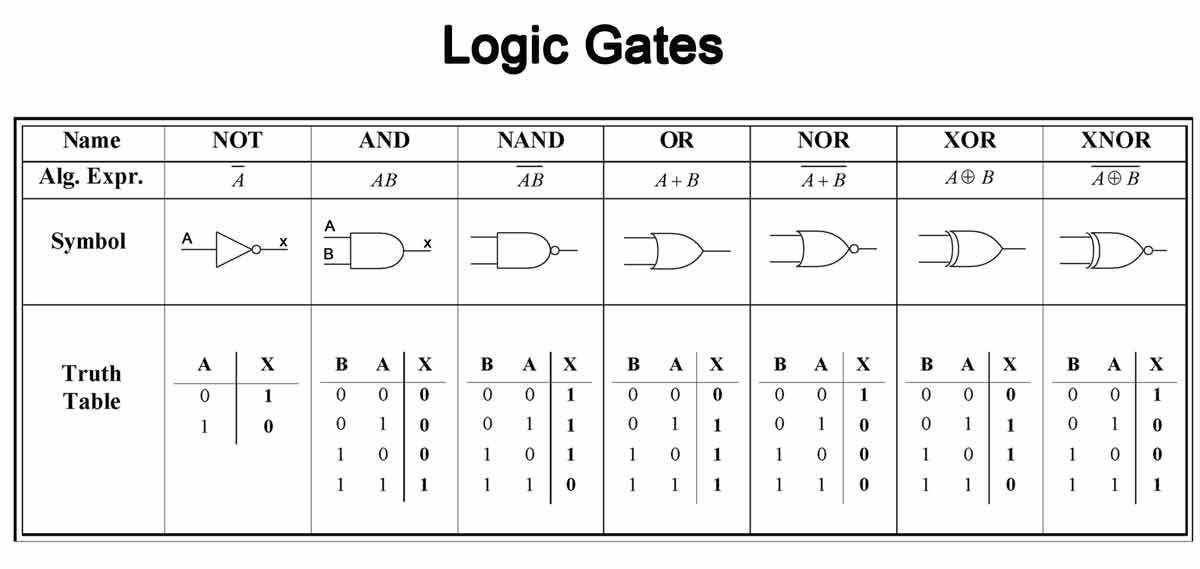
\includegraphics[width=16cm, height=8cm]{image/logic-gates.jpeg} 
    \caption{Floating Point}
    \label{logic-gates}
\end{figure}

\begin{itemize}
\item  truth table, is used to represent all possible inputs and then the corresponding output.
\item  To determined the possible schematics one can write for the input A and B ``!A and B''
  not A and B. One often get a unnecessary complexity, one can often simplify the schematics.
  It is only done with the inputs that have an output of one.
\item  De Morgan’s Law $!(A+B)=!A \cdot !B$ $+$ and $\cdot$ works the same way but are different.
\item  karno map is used to easily determine the schematics. It is a matrix. It is possible to use
  more inputs then two. In the matrix one locks at when output is one.
\item  a cabal with 4 wires can take 4 bits. Overflow needs one extra wire on output
\end{itemize}


\textbf{Building blocks}
\begin{itemize}
\item   Building blocks are the first layer of abstraction since one can not se the logical gates
  constructed of. For example add is a building block.
\item  Two types of logic, combinational and sequential.
  combinational: output just depends on input
  sequential: output deepens on the state. State is stored in memory update on clock.
\end{itemize}

\begin{itemize}
\item  MUXes (Mulitplexrs): choose input from a buss/ routing signal.
  2-bit decision for input 4-bit selection. Starts from position 0.
\item  DEMUXes (Demulitplexrs): oposit, take on signal and decides where it want to be sent to
  Buss is a multi-bit signal ``wire''
\item  Decoder: binary to hot, (adds a zero or one)? in arrays it can shose position
\item  Encoder: hot to binary, (reomve a zero or one)?
\item  Adders: adds carrys on extra bit to handel overflow
\end{itemize}

\begin{figure}[h]
    \vspace{10mm}
    \centering
    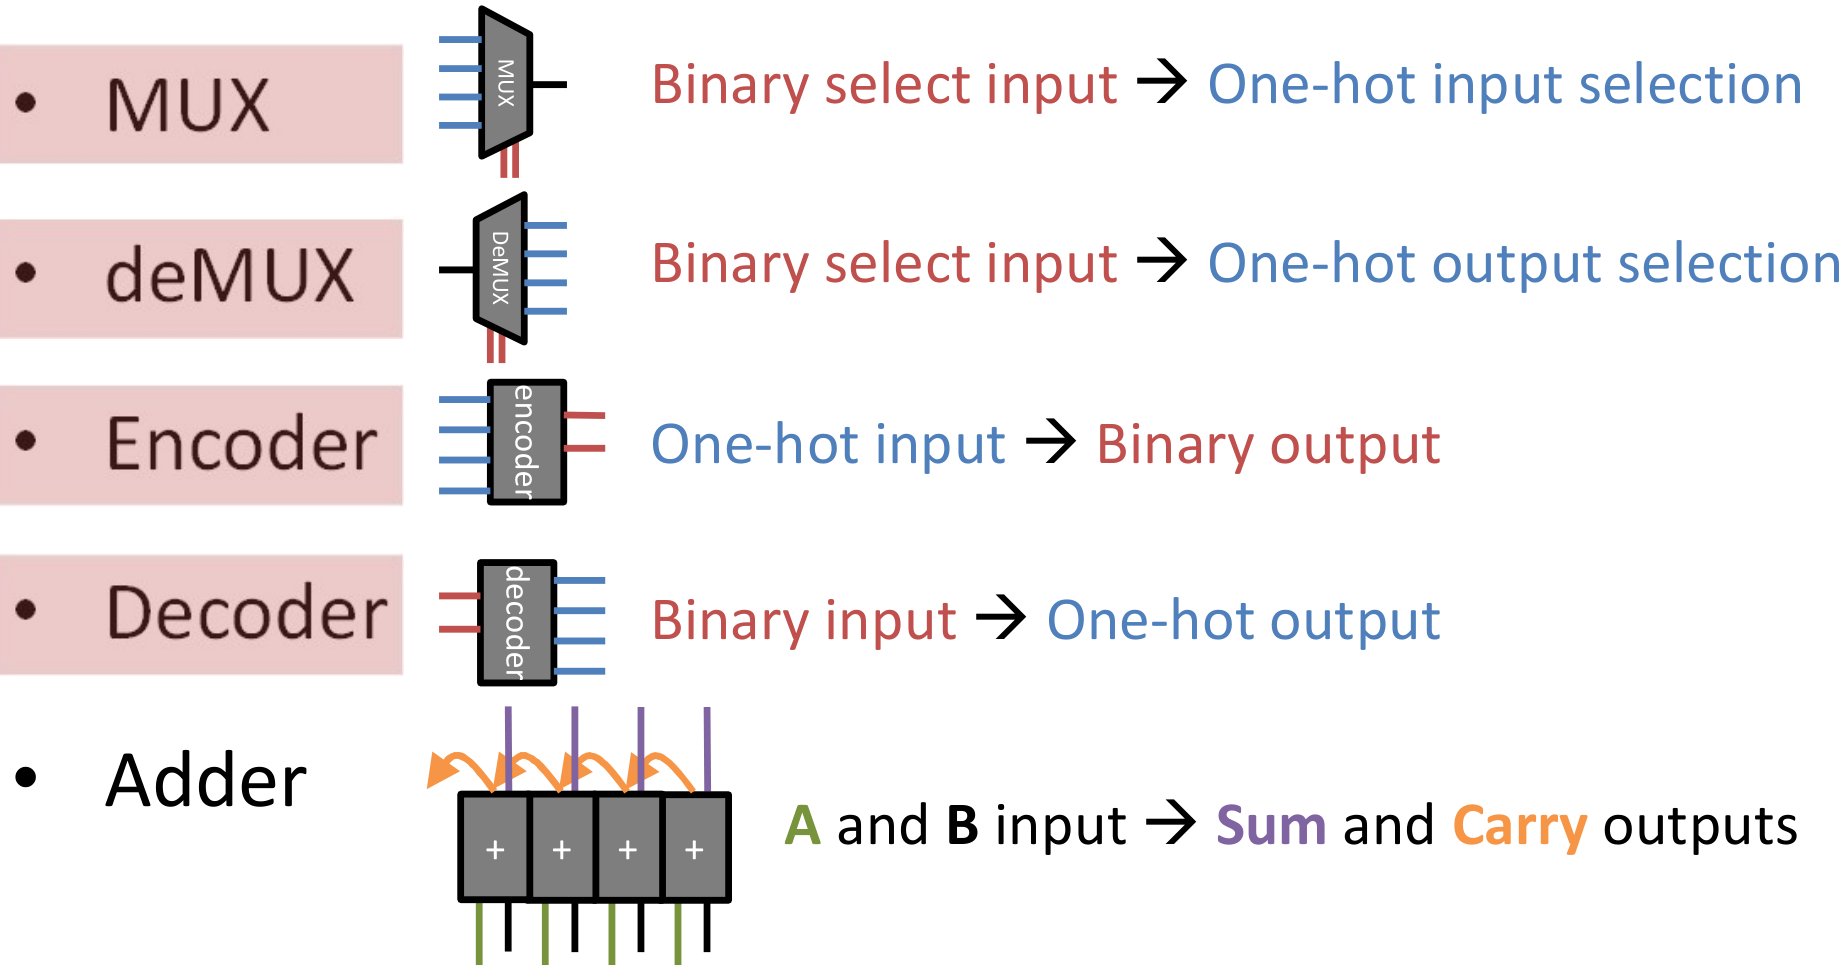
\includegraphics[width=16cm, height=8cm]{image/important-logic-blocks.png} 
    \caption{Floating Point}
\end{figure}

\textbf{Latches}
\begin{itemize}
\item  One use is for counters with a clock statest trigers the count.
  So when input is one the ouput is 0 and when the clock cliks it is one then when the input is
  0 the output is still 1.
\item flip flop: is a edge trigerd latche has a clock triger to open or close lathce and then can save it to SRAM cell
\end{itemize}

\begin{figure}[h]
    \vspace{10mm}
    \centering
    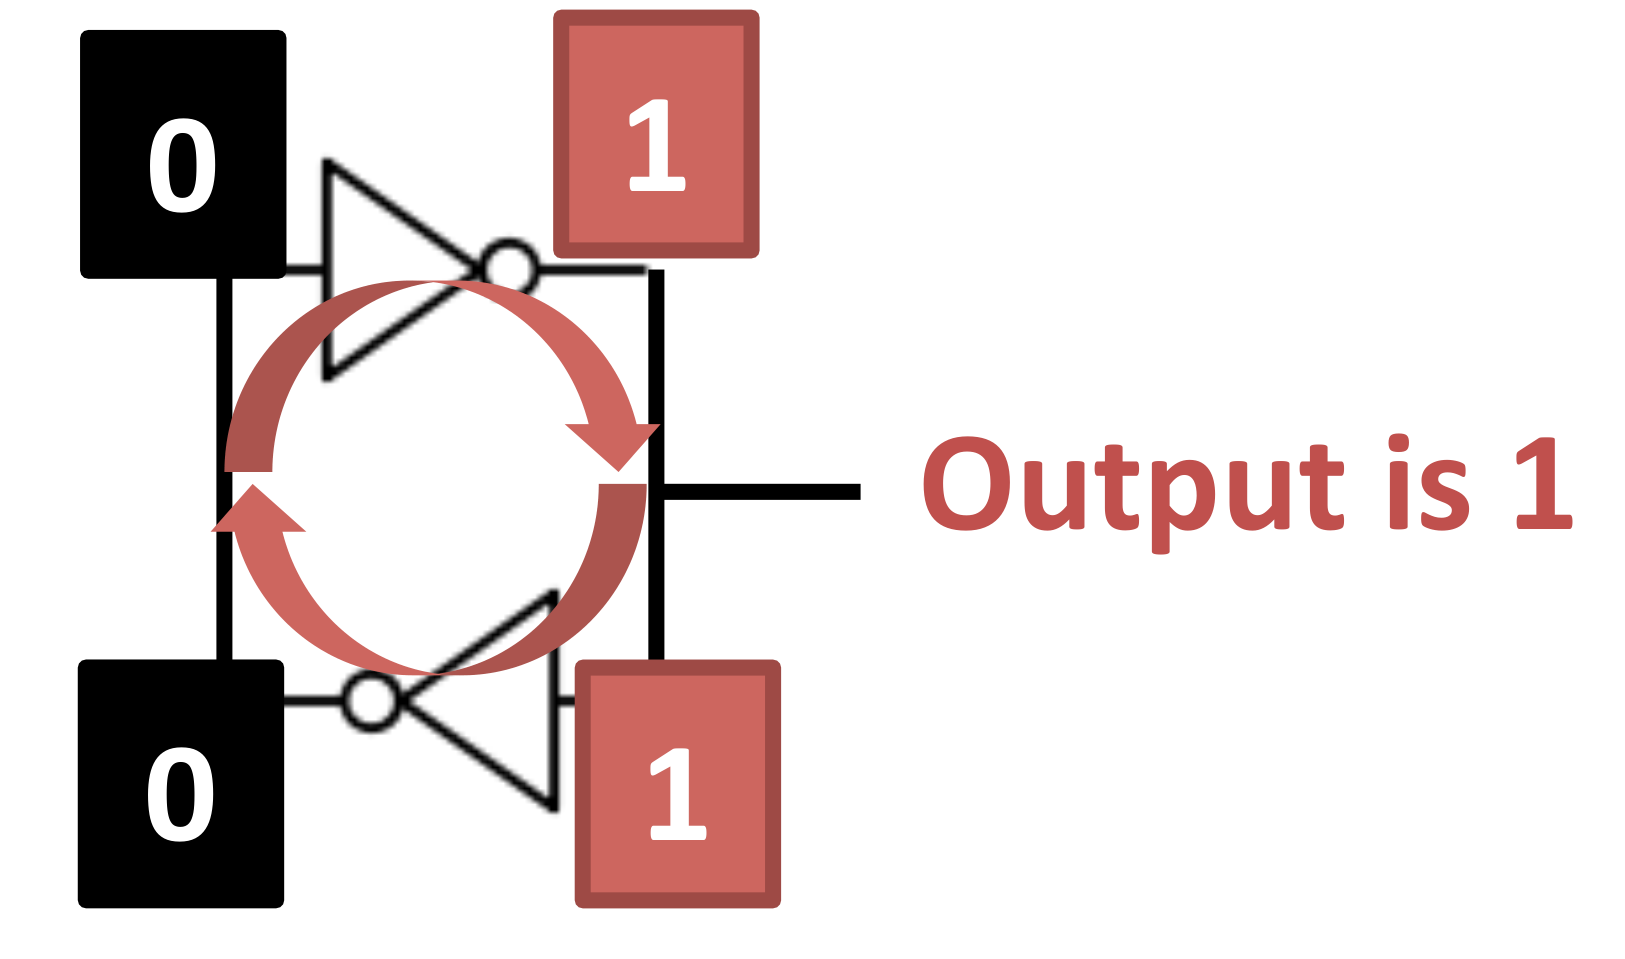
\includegraphics[width=16cm, height=8cm]{image/latche.png} 
    \caption{latche}
\end{figure}

\textbf{Memory}
\begin{itemize}
\item  SRAM (Static Random Access Memmory) Big, fast and expensive. Loops thou value in order to store it.
  To write to memory one uses a switch to update value.
\item  DRAM (Dynamic Random Access Memory) Smaller, Slower and cheaper. Uses a transistor to store value
  and a capacitor to store the charge so the data dose not disappear.
  That is why it is slower become the capacitor needed to be recharge
\end{itemize}


\newpage


\section{processor control and datapath}
There is 3 main part of the mips datapath as seen in the following image:
\begin{figure}[h]
    \vspace{10mm}
    \centering
    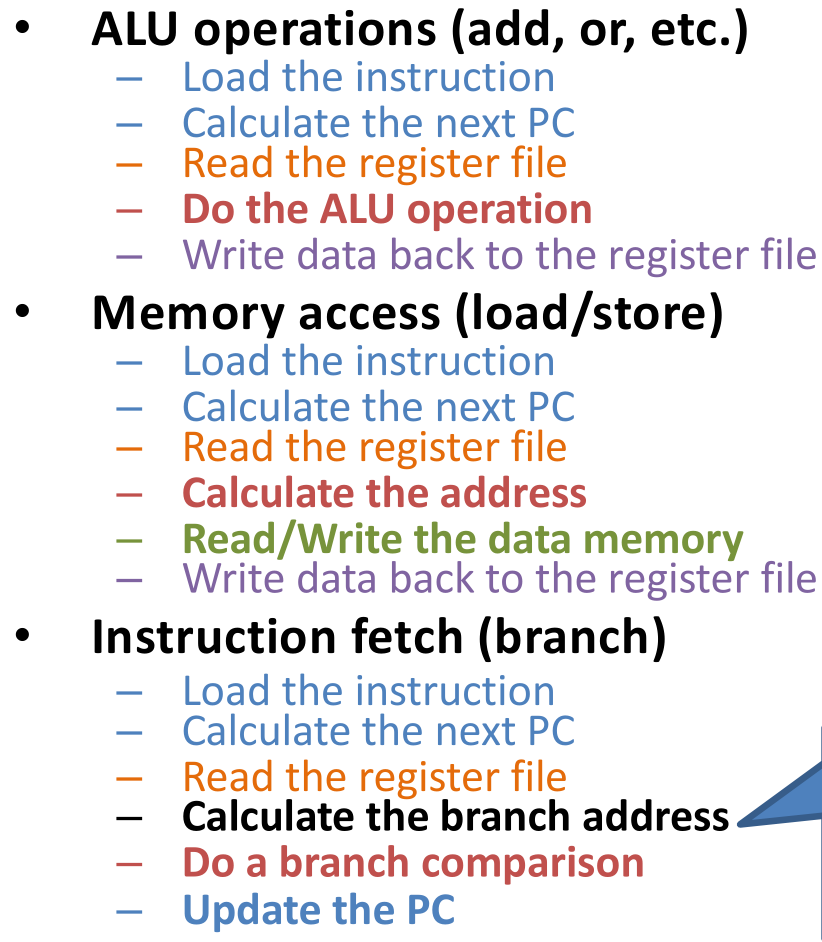
\includegraphics[width=12cm, height=14cm]{image/mips-datapath-3parts.png} 
    \caption{mips datapath 3 parts}
    \label{mips-datapath-3parts}
\end{figure}

\newpage

An overview of the mips datapath with j-format instruction:
\begin{figure}[h]
    \vspace{10mm}
    \centering
    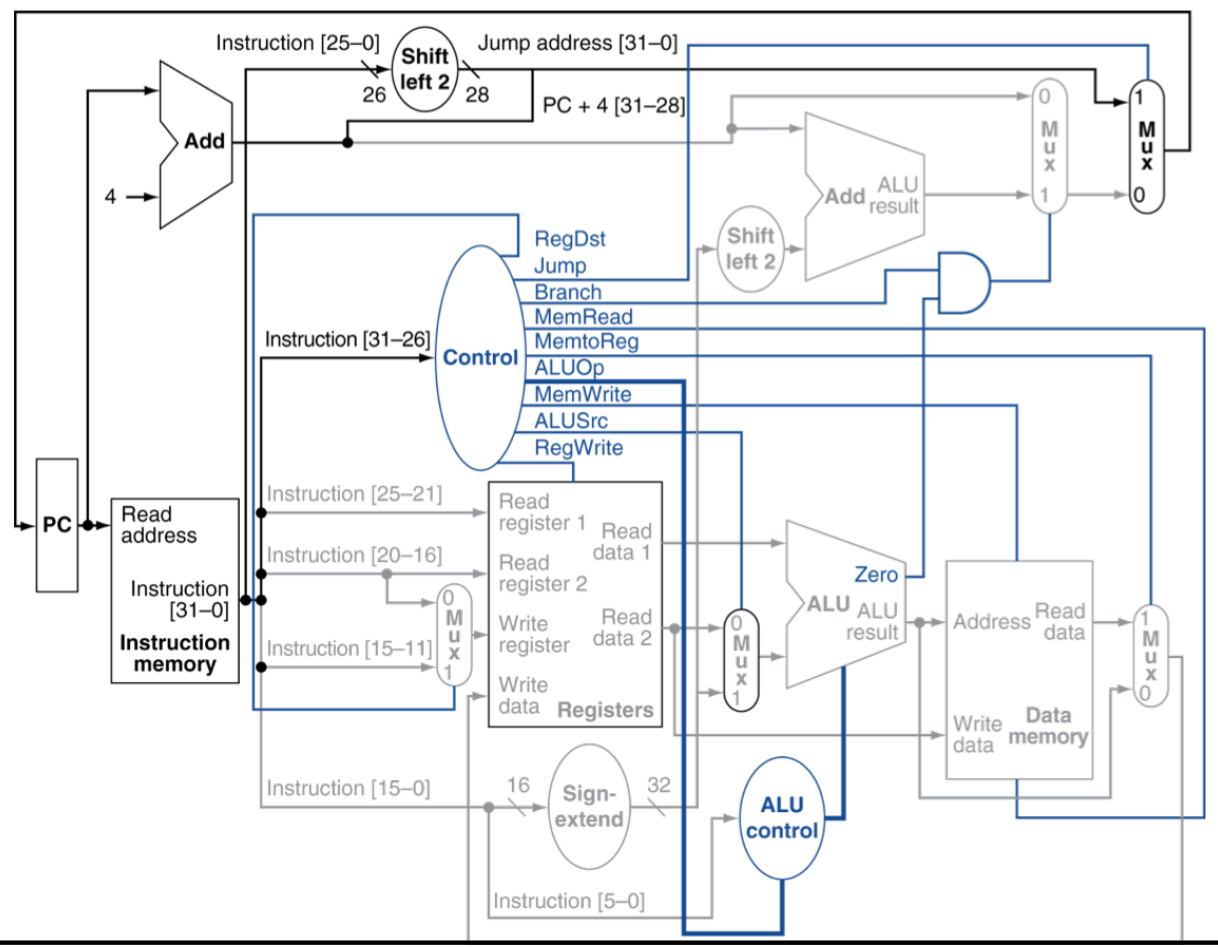
\includegraphics[width=16cm, height=12cm]{image/mips-datapath.png} 
    \caption{mips datapath}
    \label{mips-datapath}
\end{figure}

Think about the controler like a decoder that decodes the opt code from the diffrent formats.

\newpage

\subsection{Clock}
A clock is used to update the state and continu with the other instructions. Every state element uses
a clock. In mips prosesor clock gose to memory, pc, rf and dm. The clock unit is in (MHz) converting
from (ns) is simple. Ex 10ns: 1/10ns=0.1MHz.

\subsection{Critical path}
The longest path of the datapath is the critical path. Often PC is the fastest so one then calculates the
amount of time it takes for the instruciton has traveld the data path and reternd to know what the
critical path is. The longest part is data memory sinze it is big and slow. One often say read and write
takes constant time regardless of the amout of diffrent read and write.


\newpage


\section{pipline}
The perpus is to split a instruction cycle into multipe stages to run instructions in peralel to
improve preformans. Itch stage has its own pipline registerfile for storing the nessasary registers.
Pipline registers has a preforment reduction since it takes time, therfore more pipleine stages dose
not eqal greater proformens over a serten abount. One issue of preformans is balance the stages
inorder to get a good clock frequency. 
Not all stages are needed for eatch operation or instruction

\textbf{Mips stages}
\begin{itemize}
\item  IF= Instruction fetch
\item  ID= Decode and RF Read
\item  Ex= ALU Execute
\item  MEM= Memory
\item  WB= RF Write back
\end{itemize}

\begin{figure}[h]
    \vspace{10mm}
    \centering
    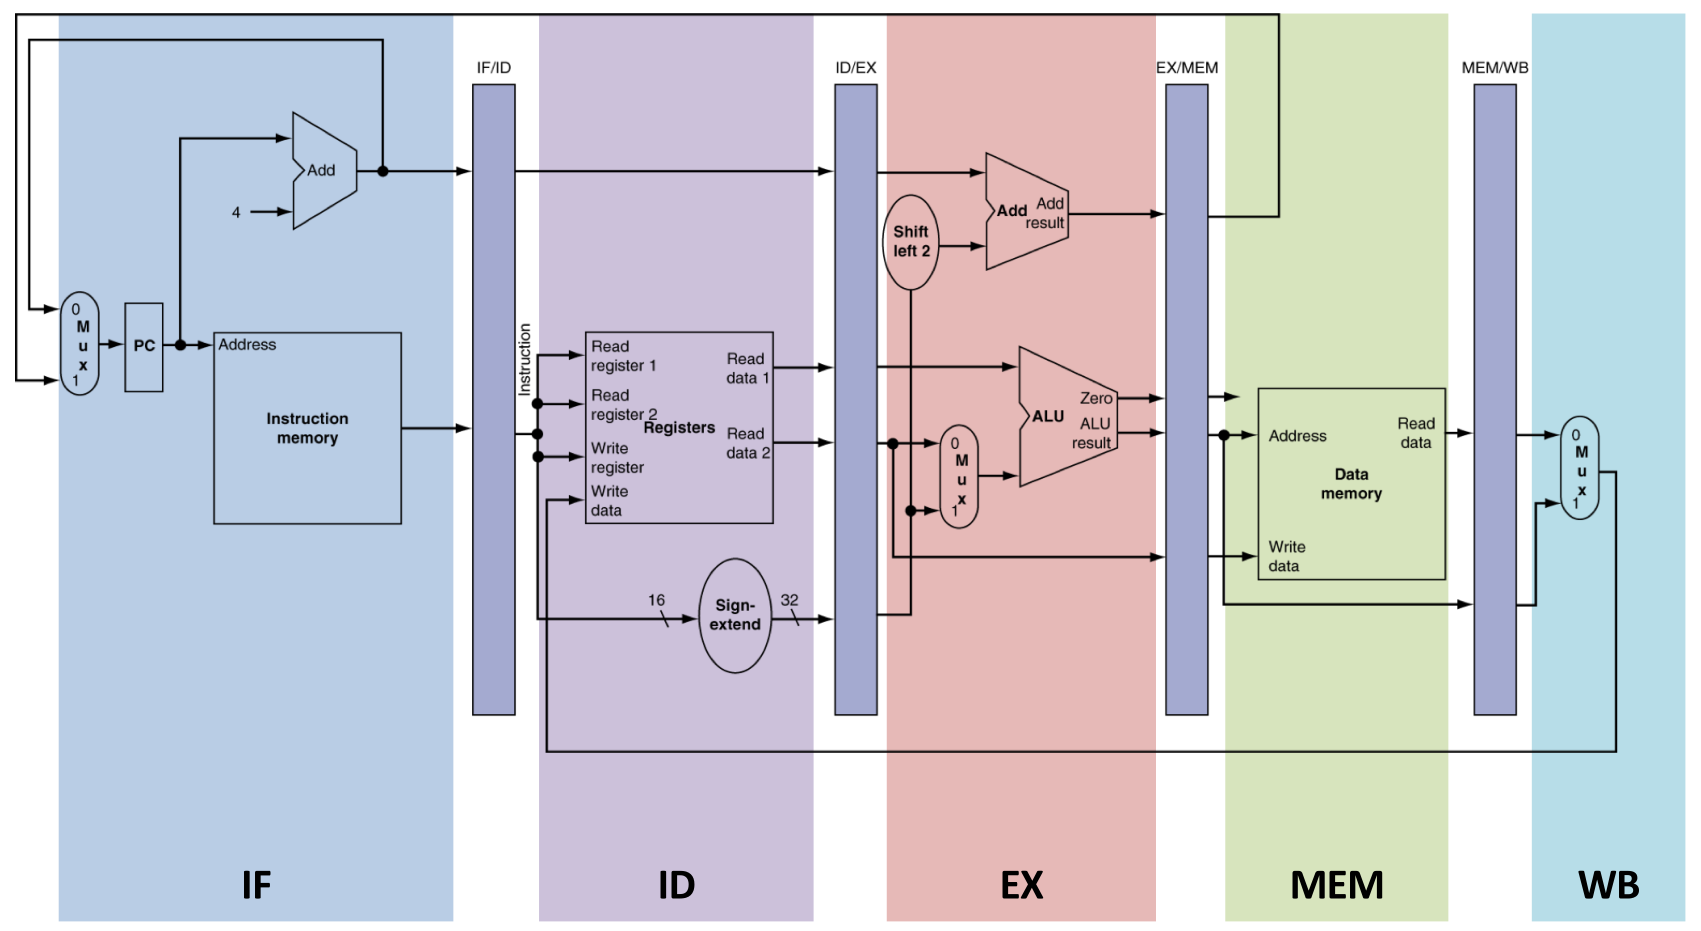
\includegraphics[width=16cm, height=8cm]{image/pipline.png} 
    \caption{Pipline}
    \label{pipline}
\end{figure}


\textbf{Terminology}
\begin{itemize}
\item  Bubbles= Is detected by the harwere where ther is no instuctions
\item  Nop= Is a sudo instruction for a stall type instruction (do not do anything)
\item  Delay slots= a stall type for branches. Try to fill in those slots with usful instructions.
\item  Interference= Can not read and write at the same time.
\item  Double pumping= Spiting write to first clock cycle and the second cycle is read.
\item  Forwarding= Getting data from a different pipeline stage from a register file.
\end{itemize}

\textbf{Calculating time coplexity}
\begin{itemize}
\item  overhead: (instructions time (ex 100ns)) / (stages (ex 1000)) + (regester overhead (1ns)) = 1.1ns \newline
    Total time: 1.1*1000
\item  Latancy: (stages* (penalty per stage) + original) \newline
  Latancy: (Time per instruction (ex 100ns)) + (pipline register's (ex 100-1))* (penalty per stage (ex 2ns)) = 300ns (3x slower)
\item  Trouput: (Time per instruction (ex 100ns))/ (Stages (ex 100-1)) + (Time pipline registes (ex 2ns)) = 3ns (every instuction is 33x faster) 
\end{itemize}


\newpage


\section{Pipline hazards}

\subsection{Data hazards}
\textbf{The issue}
\begin{itemize}
\item  Data is not available where we need it (later in the pipeline; not written back yet).
\item  Data is not available when we need it (need to read memory first).
\end{itemize}

\textbf{Fixing the issue}
\begin{itemize}
\item  Forward the data to where we need it.
\item  Stall if data is not ready yet (NOPs or Bubbles).
\end{itemize}

\begin{figure}[h]
    \vspace{10mm}
    \centering
    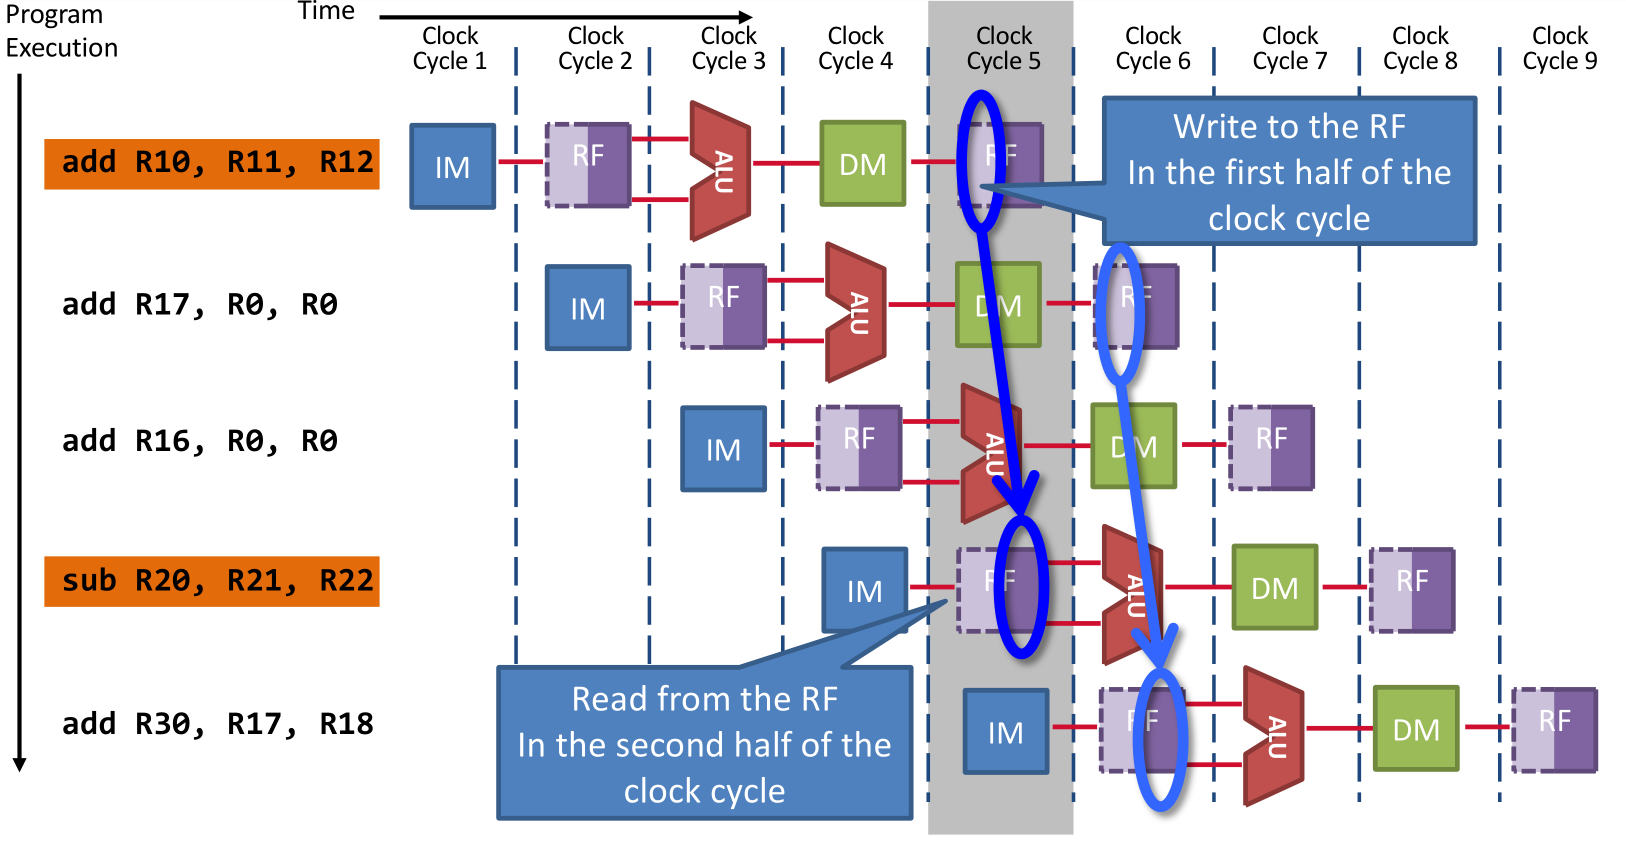
\includegraphics[width=16cm, height=8cm]{image/dubble-pump.png} 
    \caption{Dubble pump}
\end{figure}


\subsection{Control hazards}
\textbf{The issue}
\begin{itemize}
\item  Don’t know which instruction is next when we need to fetch it.
\end{itemize}

\textbf{Fixing the issue}
\begin{itemize}
\item  Calculate branch as early as possible.
\item  Stall with a branch delay slot.
\end{itemize}


\subsection{Structural hazards}
\textbf{The issue}
\begin{itemize}
\item  Can’t do the instruction because the hardware is busy.  
\end{itemize}

\textbf{Fixing the issue}
\begin{itemize}
\item  Build more hardware (double-pumped register file).
  Double-pumped write at the first hafe cycle and read at the other half
\end{itemize}

\textbf{Calculating time coplexity}
\begin{itemize}
\item  Branshe delay \newline
  (How many branches (ex 20\%)) / (How maney usful instuctions can be filled in (ex 50\%))
  = 20\%/0.5 = 10\%
\item  Cycles per instructions (CPI): (total cycles (with nop)) / (usful work (without nop))
  % https://www.youtube.com/watch?v=GAUppsLpjvg
\end{itemize}
%The amount of instructions that requires a NOP is 50% of 20% = 10% => 10% of instructions will take 2 cycles 
%This gives us a CPI of 10%*2+90%*1 = 0.1*2+0.9*1 = 1.1 CPI 
%Therefore, the slowdown due to the load delay-slots is 10%.


\newpage


\section{Predicting Branches and Exceptions}
When the prediction is wrong, clean up is needed.
– “Kill” or “Squash” so they don’t execute (they were wrong)
– Prevent them from writing: disable RegWrite, MemWrite in the pipeline
– Turn them into NOPs: change opcode to add R0, R0, R0 in the pipeline


\subsection{Static pridictors}
\begin{itemize}
\item  Predict alwas not taken
\item  Predict alwas taken
\item  Backwards-Taken, Forward-Not-Taken (BTFNT)
\end{itemize}


\newpage


\subsection{Dynamic pridictors}

The implementation of branch preditors look somthing like this:
\begin{figure}[h]
    \vspace{10mm}
    \centering
    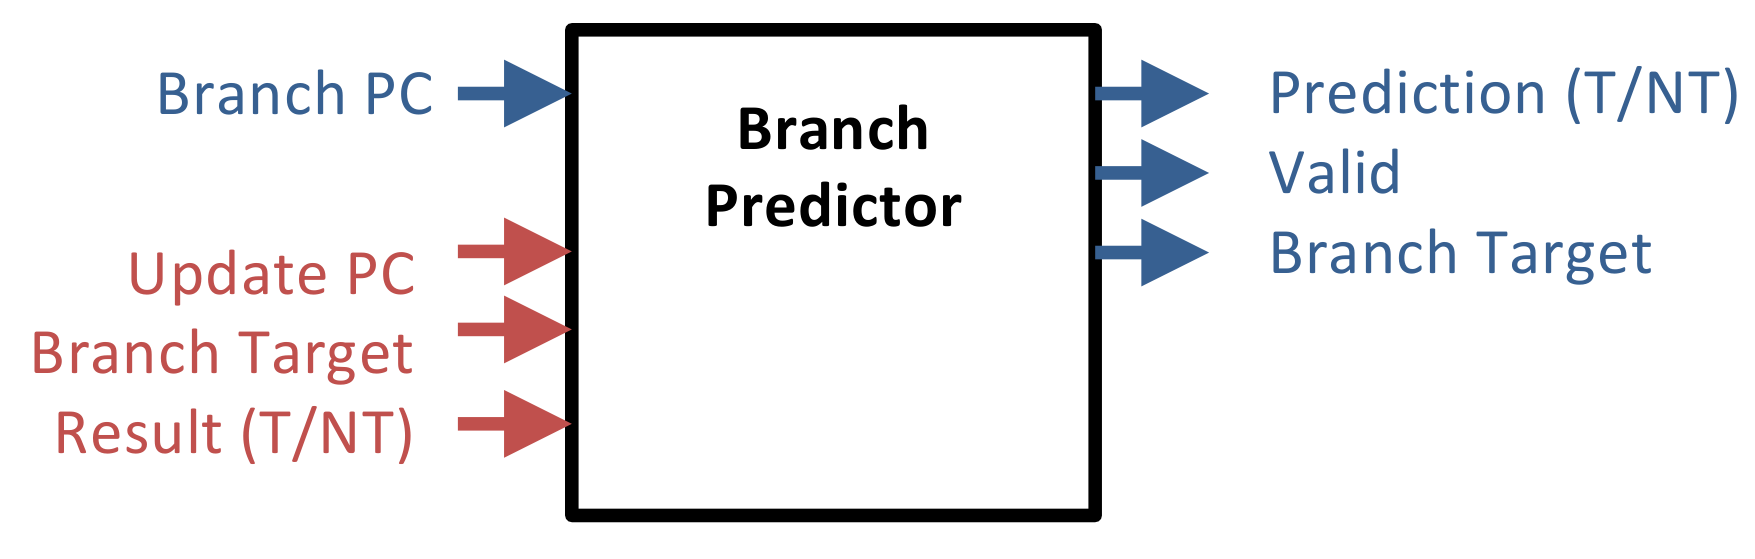
\includegraphics[width=16cm, height=5cm]{image/branch-predictor.png} 
    \caption{branch-predictor}
\end{figure}


\begin{figure}[h]
    \vspace{10mm}
    \centering
    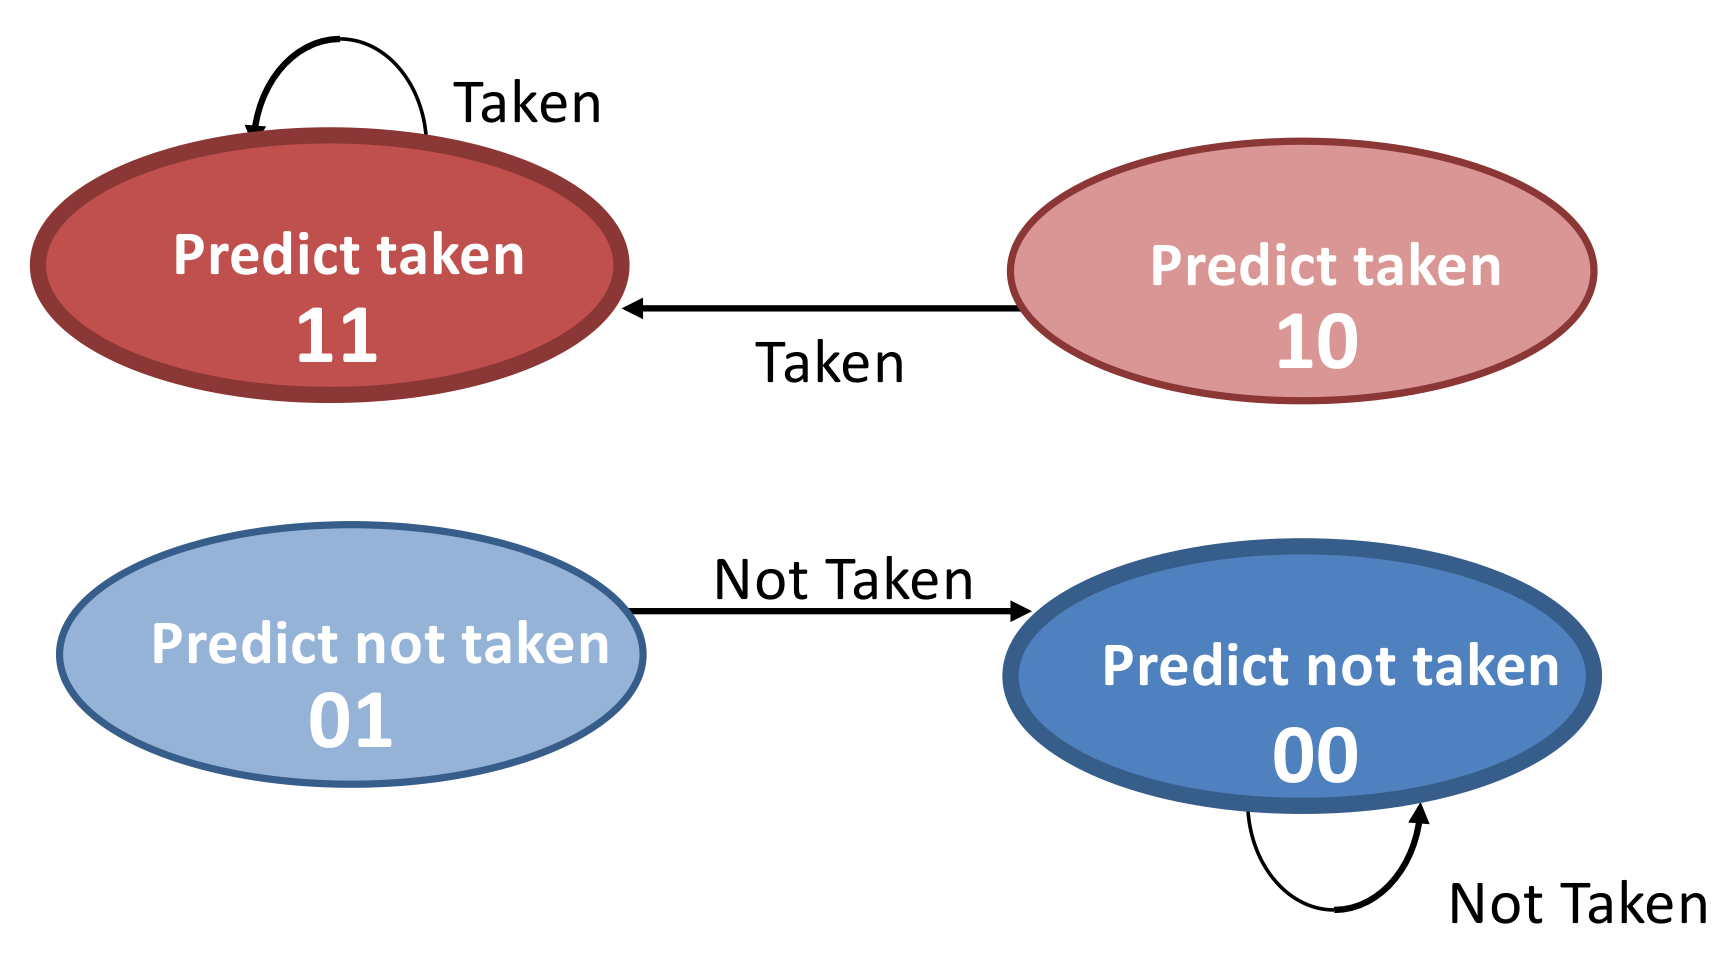
\includegraphics[width=16cm, height=10cm]{image/2-bit-predict.png} 
    \caption{2-bit predict}
\end{figure}

\newpage

\textbf{BTB}
\begin{itemize}
\item  Branch Target Buffer (BTB)
\item  Save a table with PC onorder to have history that we can predict on
\end{itemize}

\begin{figure}[h]
    \vspace{10mm}
    \centering
    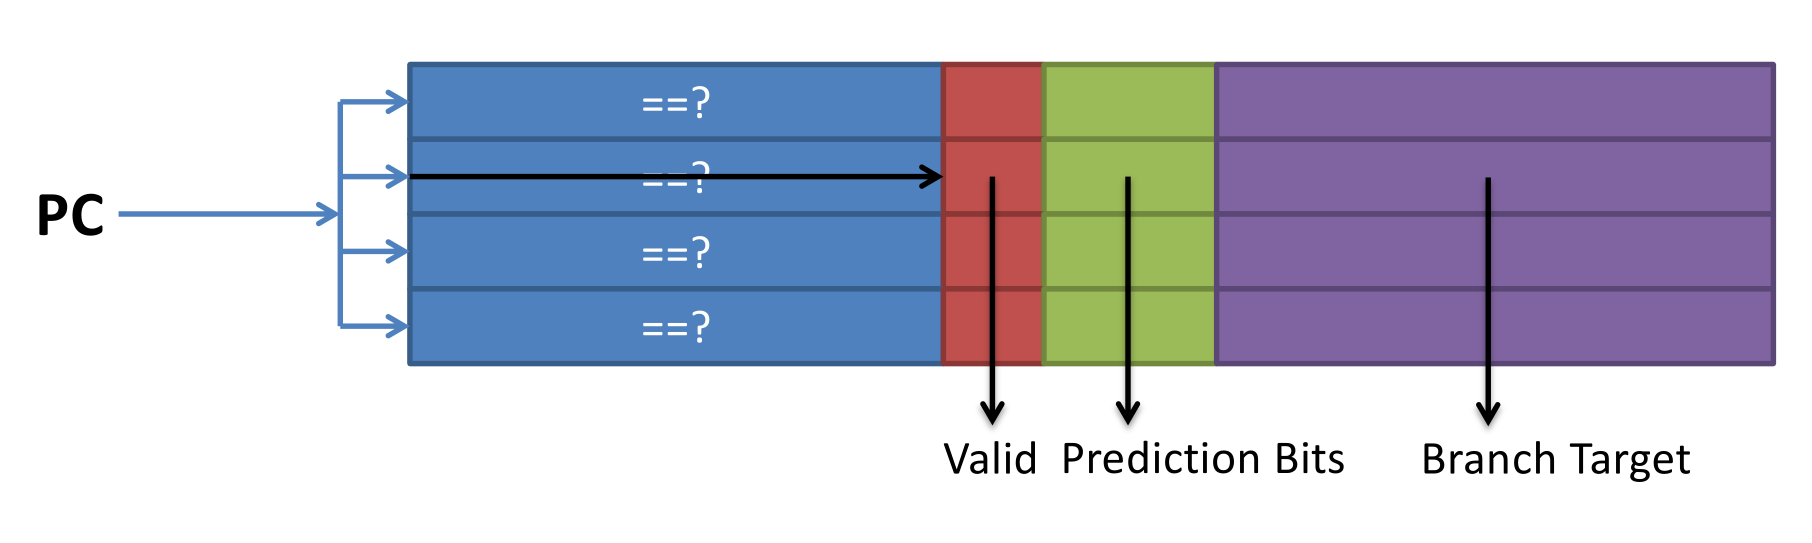
\includegraphics[width=16cm, height=5cm]{image/btb.png} 
    \caption{btb}
\end{figure}


\newpage

\subsection{Exceptions}
Exceptions are non-normal events that interrupt the normal flow of instructions
\begin{itemize}
\item  Divide by zero
\item  Misaligned memory access
\item  Page fault
\item  Memory protection violation
\end{itemize}

Interrupts are external events that interrupt the normal flow of 

\begin{figure}[h]
    \vspace{10mm}
    \centering
    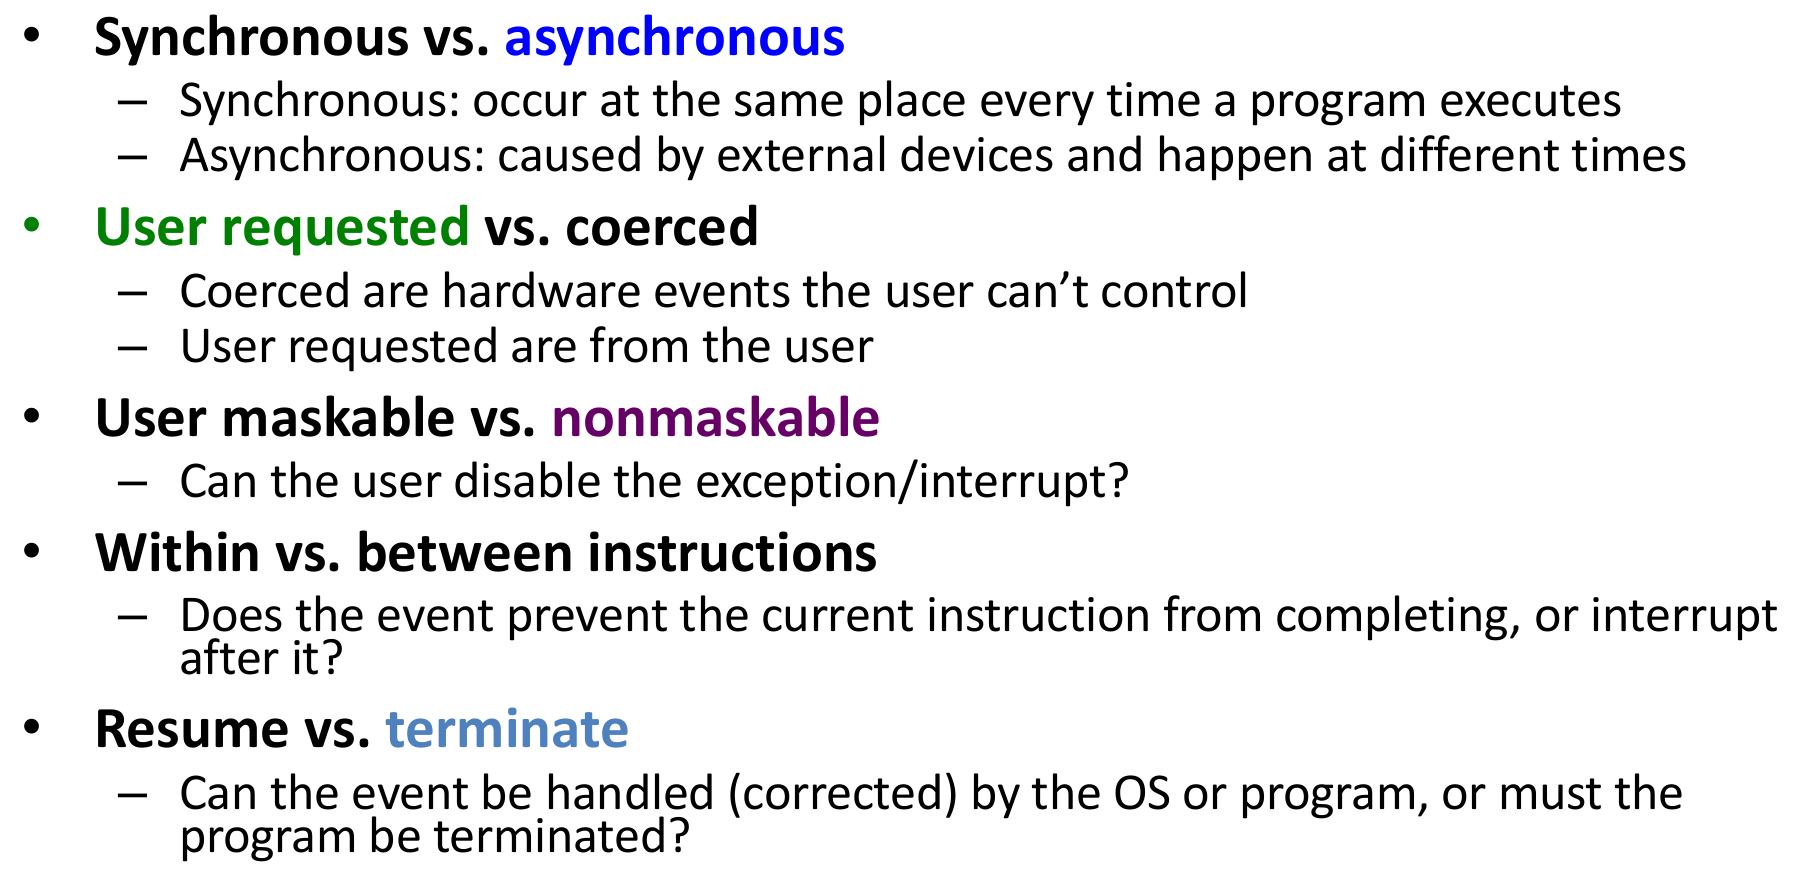
\includegraphics[width=16cm, height=9cm]{image/exceptions.png} 
    \caption{exceptions}
\end{figure}


\newpage


\section{Input/Output}

\textbf{Terminology}
\begin{itemize}
\item  nvram (flash): Simmiler to ram but it saves data when there is no power
\item  Busses:
  Parallel: many bits at once (e.g., 32 bits together in one clock)
  Used to be used everywhere
  Still used inside chips
\item  Serial links:
  Serial: one bit at a time (e.g., 32 clock cycles to send 32 bits)
  Used to be used only where distances were long (e.g., networks)
  Now used for most off-chip communications
\item  memory-mapped I/O:
  Manual handeling of I/O devices
  Map portions of the address space to I/O devices
  Read and write to those addresses to access the 
\item  direct memory access (DMA):
  Hardware who mange I/O devices (dynamicly)
\item  Polling:
  The device puts its status somewhere
  The OS repeatedly checks for it to change
\item  Interrupt:
  When the device is ready, it gets the processor’s attention by signaling an interrupt
  The OS then jumps to an interrupt handler to handle the event
\item  Througput: x/s
  The read and write speed
\item  Lateny: s/x
  Accesing time.
\item  Overhead:
  any combination of excess or 
  indirect computation time, memory, bandwidth,
  or other resources that are required to perform a specific task
\end{itemize}


\newpage

\textbf{Data transfers: manual copy}
\begin{lstlisting}%[language=Assembly]
addi R3, R0, 921600  // Number of copies
add   R2, R0, R0      // Counter starts at 0
loop:
  lw R4, 0x12f0(R0)  // Read the I/O device
  sw R4, 0xfe00(R2)  // Store the results
  addi R2, R2, 4       // Next location
  bne R3, R2, loop
done:
\end{lstlisting}


\textbf{Data transfers: DMA}
\begin{lstlisting}%[language=Assembly]
addi R1, R0, 0x12f0 // device address
addi R2, R0, 0xfe00 // destination
addi R3, R0, 230400  // number of words to copy
sw R1, 0x100b(R0) // set the device address
sw R2, 0x1008(R0) // set the destination address
sw R3, 0x1004(R0) // set the length and start
wait:
  lw R2, R0(0x1000) // Wait for it to be done
  bne R2, R0, wait
done:
\end{lstlisting}


\newpage


\section{Cache}
\subsection{Memory hierarchy}

\begin{figure}[h]
    \vspace{10mm}
    \centering
    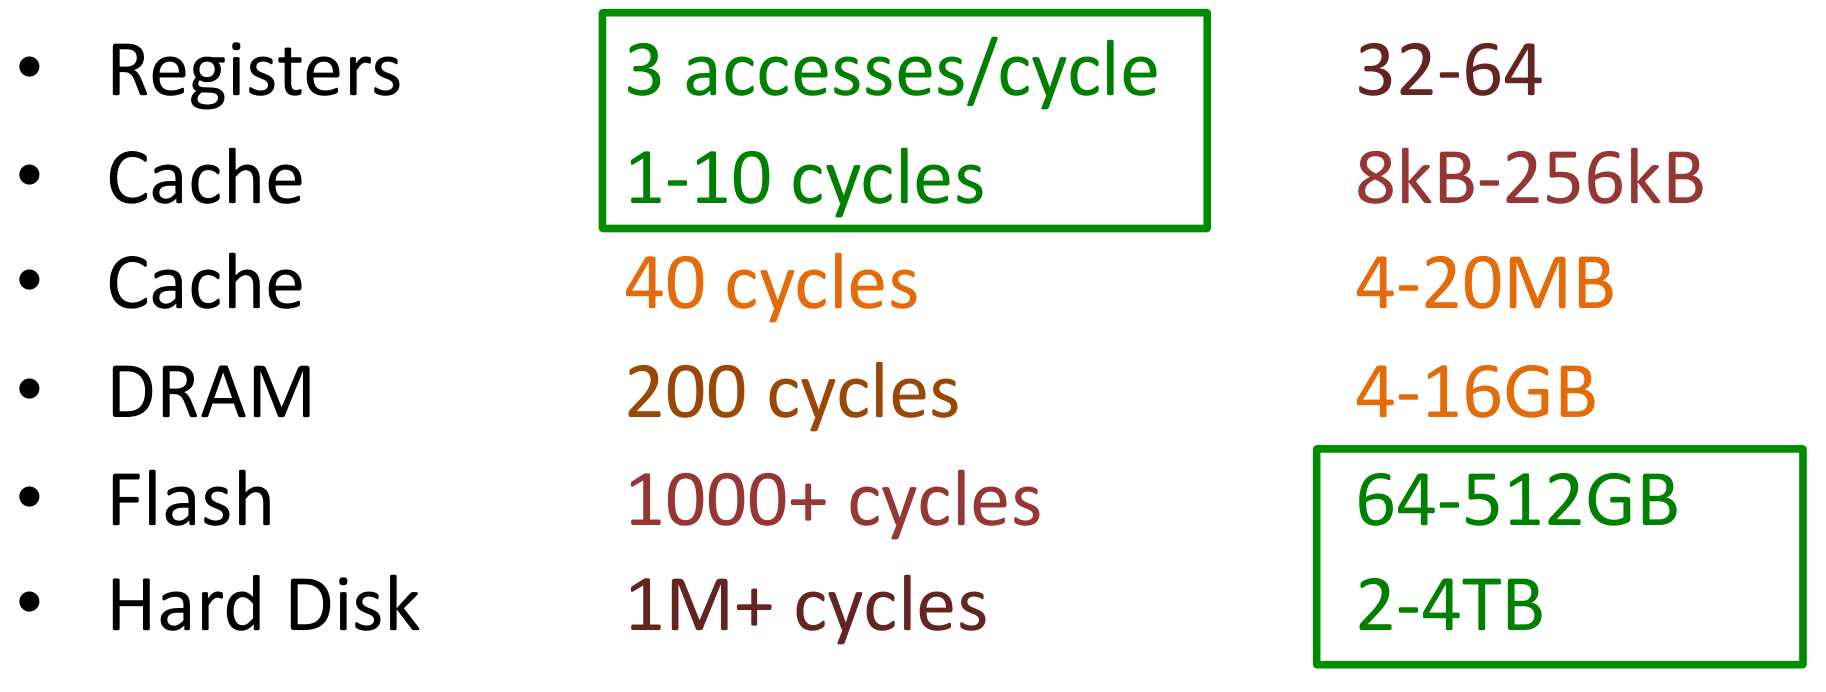
\includegraphics[width=16cm, height=7cm]{image/memory-hierarchy.png}
    \caption{memory-hierarchy}
\end{figure}

\textbf{3-types of cache types}
\begin{itemize}
\item  Fully-associative: Have to search all blocks, but very flexible 
\item  Direct-mapped: Only one place for each block, no flexibility
\item  Set-associative: Only have to search one set for each block,
  flexible because each set can store muliple blocks in its ways 
\end{itemize}

\textbf{Write policies}
\begin{itemize}
\item  Write-through: slow, simple 
\item  Write-back: fast (keeps the data just in the cache), more complex
\end{itemize}

\textbf{Termenology}
\begin{itemize}
\item  Data: What is being stored
\item  Tag: What address the data has
\item  Index: What we use to determen where we want to put the data
\item  Cache line (block) size: How many tag's there are
\item  Valid bit: If the data is correct
\item  Dirty bit: The data has been change and we need to write it to memory
\item  Type of cache: Fully-associative (FA), Set-associative (SA), Direct-mapped (DM)
\item  Replasment policy: Write-through, Write-back  
\end{itemize}


\textbf{Cache blocks}
\begin{itemize}
\item tag has 30bits and the 2 other bits is to determen what data
  63 bits for eatch entry 32bit data 30bit tag 1bit valid-bit 
\item larger block of data -> fewer tags -> more effeciant storage
\item 1 word cache block we have 1 32bit data
\item 2 word cache block we have 2 32bit data 
\item 4 word cache block we have 4 32bit data
\item we loade more data when we have space for it
  we will then have spatial locality
\item Last 2: determine the byte within the word   
\item Next N: determine which word in the cache block 
\item Remaining 32-N-2: tag
\end{itemize}

\textbf{Calculate overhead}
\begin{itemize}
\item  Data= Cache-Lines * Byte-Lines
\item  Overhead= Cache-Lines * (Tags-per-line + valid-bit)
\item  \% data=  Overhead / Data
\end{itemize}

\textbf{Calculate Address (Tag Index Offset)} %https://cs.stackexchange.com/questions/13356/how-to-calculate-the-number-of-tag-index-and-offset-bits-of-different-caches
\begin{itemize}
\item  Direct maped: \newline
  Offest= $\log$ (number of data blocks)  (+ 2-bit (4-bite cache block size if 64 then log 64)) \newline
  Index= $\log$ (number of cache lines) \newline
  Tags= 32(bit processor)- (Index+Offset) 
\item  x-set associative: \newline
  Offest= $\log$ (number of data blocks)  (+ 2-bit determens how the address looks like) \newline
  Index= $\log$ ((number of cache lines)/x) \newline
  Tags= 32(bit processor)- (Index+Offset)
\item  fully associative: \newline
  Offest= $\log$ (number of data blocks)  (+ 2-bit determens how the address looks like) \newline
  Index= 0 \newline
  Tags= 32(bit processor)- (Offset)
\end{itemize}

\begin{figure}[h]
    \vspace{10mm}
    \centering
    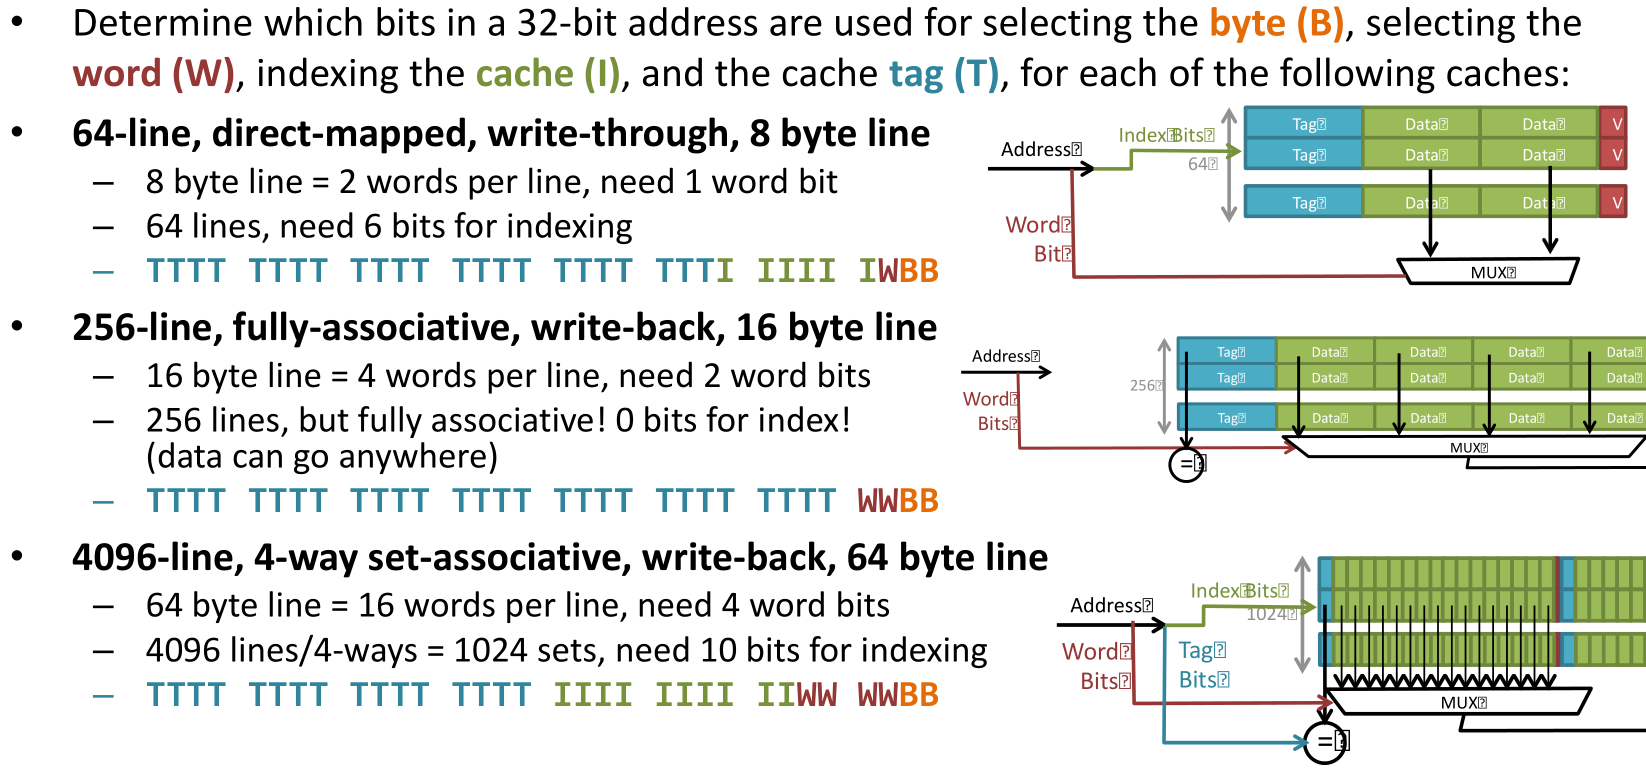
\includegraphics[width=16cm, height=7cm]{image/cache-format.png}
    \caption{cache-format}
\end{figure}


\textbf{Calculate Avrage memory access time}
\begin{itemize}
\item  Avrage-cycles= CacheL1*Cycles + CacheL2*Cycles + Dram*Cycles
\end{itemize}

\textbf{Mimimum assositivity}
\begin{itemize}
\item  (page size)/  ((Cache size)/ (bytes per line)) \newline
  ex: 8kB page size 64KB cache and 32bytes per line. log $(2^{13}/ (2^{10}/32)) = 8$  therfore 8-way
\end{itemize}

\subsection{Cache misses $3C's$}
% https://www.youtube.com/watch?v=OBp7rpdg_IQ
\begin{itemize}
\item  cold/compulsory miss: When the program first begin it dosent have enything in the cache
\item  conflicts miss: to small to store the nessesary data
\item  capasity miss: mapes at the same block an then overite unessesarly 
\end{itemize}


\newpage


\section{Virtual Memory}
\textbf{Why use VM}
\begin{itemize}
\item  Map memory to disk (“unlimited” memory)
\item  Keep programs from accessing each other’s memory (security)
\item  Fill holes in the RAM address space (efficiency)
\end{itemize}

\textbf{Termonology}
\begin{itemize}
\item  Translation= map address
\item  Page tables= for each program keep track of all translations
\item  Fine grain= page table with spesific address
\item  Coarse grain= page table with adress maped ranges
\item  Page Table Entries (PTEs)= number of translation  
\item  Translation Lookaside Buffer TLB= All of the pages, fast translation via hardware
\item  VA= Virtual program addresses
\item  PA= Physical RAM addresses
\item  Page offset= point to a range and then use the offset to determen where
\item  Translation Lookaside Buffer (TLB)= page table cache (Faster)
\item  Multilevel page table translation= page table point to other page tables (inseption)
\end{itemize}

\newpage

\textbf{Combining TLB and cache}
\begin{itemize}
\item  Physical caches: slow and needs the translation first and then save get the PA
  also known as Pysical-Index, Physical-Tagged (PIPT)
\item  Virtual caches: fast uses only virtual addresses, no translation, difficult for protection
  also known as Virtual-Index, Virtual-Tagged (VIVT):
\item  Virtual-Index, Phisically-Tagged (\textbf{VIPT}): VA for index PA for tags, fast dose translation and
  fetch from cache at the same time, most commonly used.
  We need a comperitor to se if the PA tags from cache matches the TLB PA onlny then we can say if we had a hit or a miss.
  The VA offset is what the PA tag is selected and the VA tag (number of virtual pages) is what the TLB uses.
  Mostly used for L1 cache not L2.
\end{itemize}

\textbf{TLB}
\begin{figure}[h]
    \vspace{10mm}
    \centering
    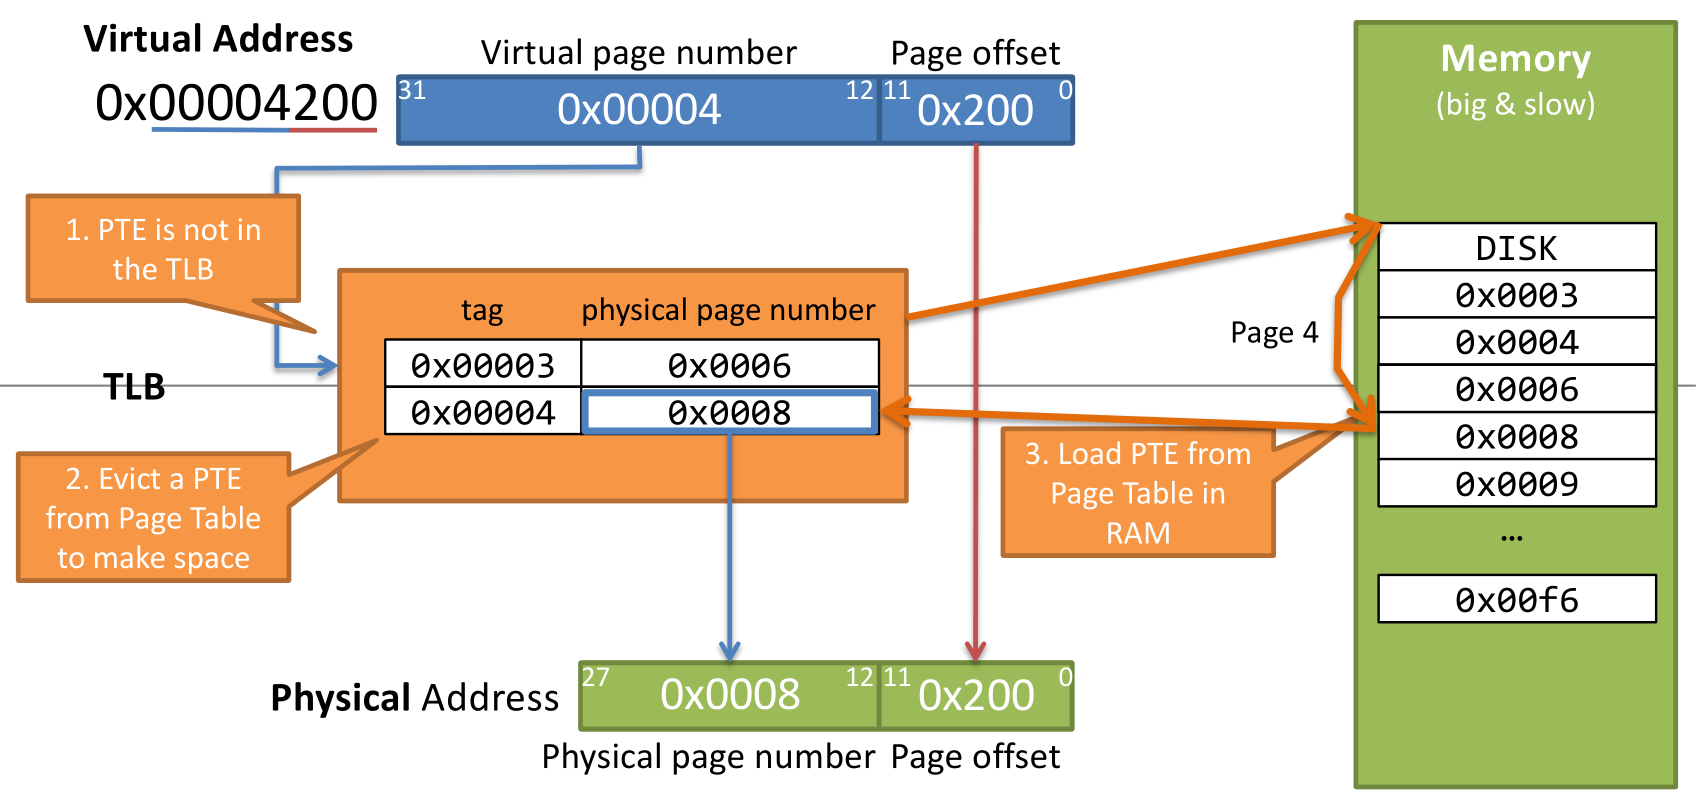
\includegraphics[width=16cm, height=7cm]{image/tlb.png}
    \caption{tlb}
\end{figure}

\newpage

\textbf{usful conversion: $2^n=xB$}
\begin{figure}[h]
    \vspace{10mm}
    \centering
    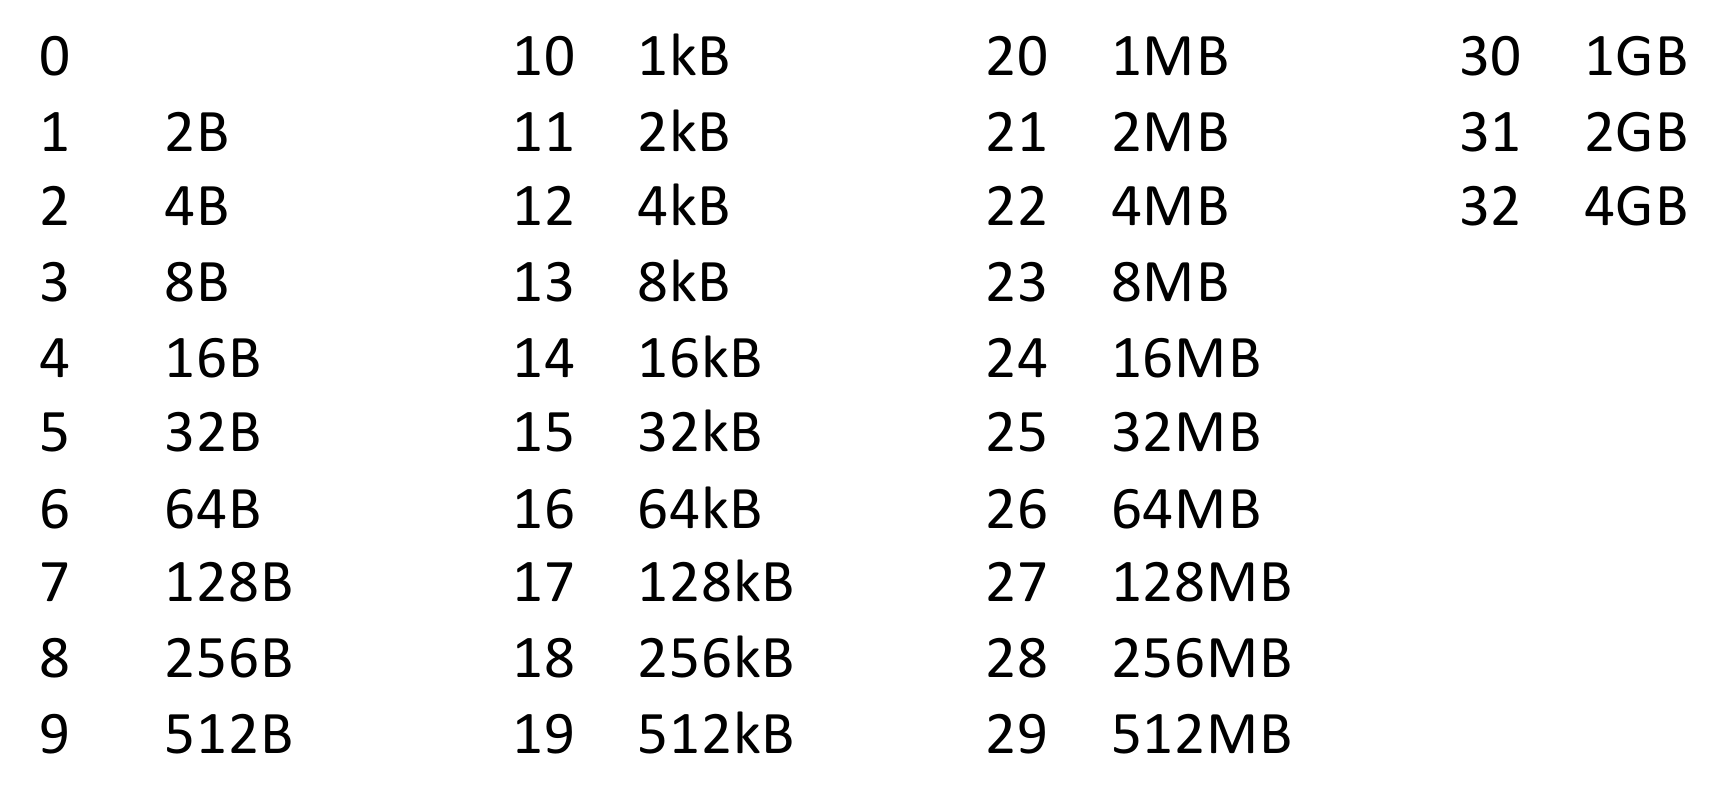
\includegraphics[width=16cm, height=7cm]{image/conversion.png}
    \caption{conversion}
\end{figure}


\textbf{Calculating Page sizeing VIPT}
\begin{itemize}
\item  Number-of-Virtual-Pages= $2^{32}/(pages)$  (in a 32bit address)
\item  Bits-used-for-Page-Offset= $\log$(pages)
\item  Bits-used-for-VPN= 32(bit prossessor)- Bits-used-for-Page-Offset
\end{itemize}

\textbf{Calculating TLB size}
\begin{itemize}
\item  TLB-size=Entries*Pages
\end{itemize}


\newpage


\section{Parallism}

\subsection{Multicore}
\textbf{powerwall}
\begin{align*}
  &\quad P=CV^2f \\
  &\quad C= \text{ capasiter, smaller transistors smaller capasiters} \\
  &\quad V= \text{ voltage, decressing makes it slower} \\
  &\quad f= \text{ frequancy, redusing clockspeed} \\
\end{align*}

\subsection{Paralel programing}


\textbf{Avrage prosessors}
\begin{align*}
  &\quad  \text{Calculate how many cores are used in avrage we need to know } \\
  &\quad  \text{how chunks (work) there is in total } \\
  &\quad  \text{how many time units (cycles think of a reverste peramid)} \\
  &\quad  \\
  &\quad  \text{there is 16 input data and we have 8-cores, we want to calculate the total sum} \\
  &\quad  \text{what is the avrage prossesor being used} \\
  &\quad  15 chunks, \; 4 time units \Rightarrow 15/4 = 3.75 \\
\end{align*}

\textbf{parallel issues}
\begin{itemize}
\item  Most programs can not utalise parellelism, need to devid the program to diffrent exicutions.
\item  We also need to share cache and therefore have proformanshe issue since we cant use the entire cache.
\end{itemize}


\textbf{How mutch faster}
\begin{align*}
  &\quad  75\% parallel, \; 25\% non parallel \text{ we have hundred thousend cores } \\
  &\quad  \Rightarrow  \text{Parallaism takes } (0.75/100000 + 0.25*1) \\
  &\quad  \text{Singuler takes } (0.75*1 + 0.25*1)  \Rightarrow 4* \text{ faster} \\
  &\quad  \\
  &\quad  \text{Speedup with Amdahl's law } Speedup=\frac{1}{(1-P)+P/S} \\
  &\quad  P= \text{ Parallel aktion} \\
  &\quad  S= \text{ Speed up of the parrallel part} \\
  &\quad  \Rightarrow \frac{1}{(1-0.75)+0.75/100000} = \frac{1}{0.25+0}= 4 \\
\end{align*}
%\subsection{Multicore issues}


\subsection{Syncronaziation}
\begin{itemize}
\item  Fix the issue with 2 prosessors accesing the same value att the same time.
\item  We can use atomic swap to first set lock to 1 then check the data.
\end{itemize}

\newpage

\textbf{locks}
\begin{figure}[h]
    \vspace{10mm}
    \centering
    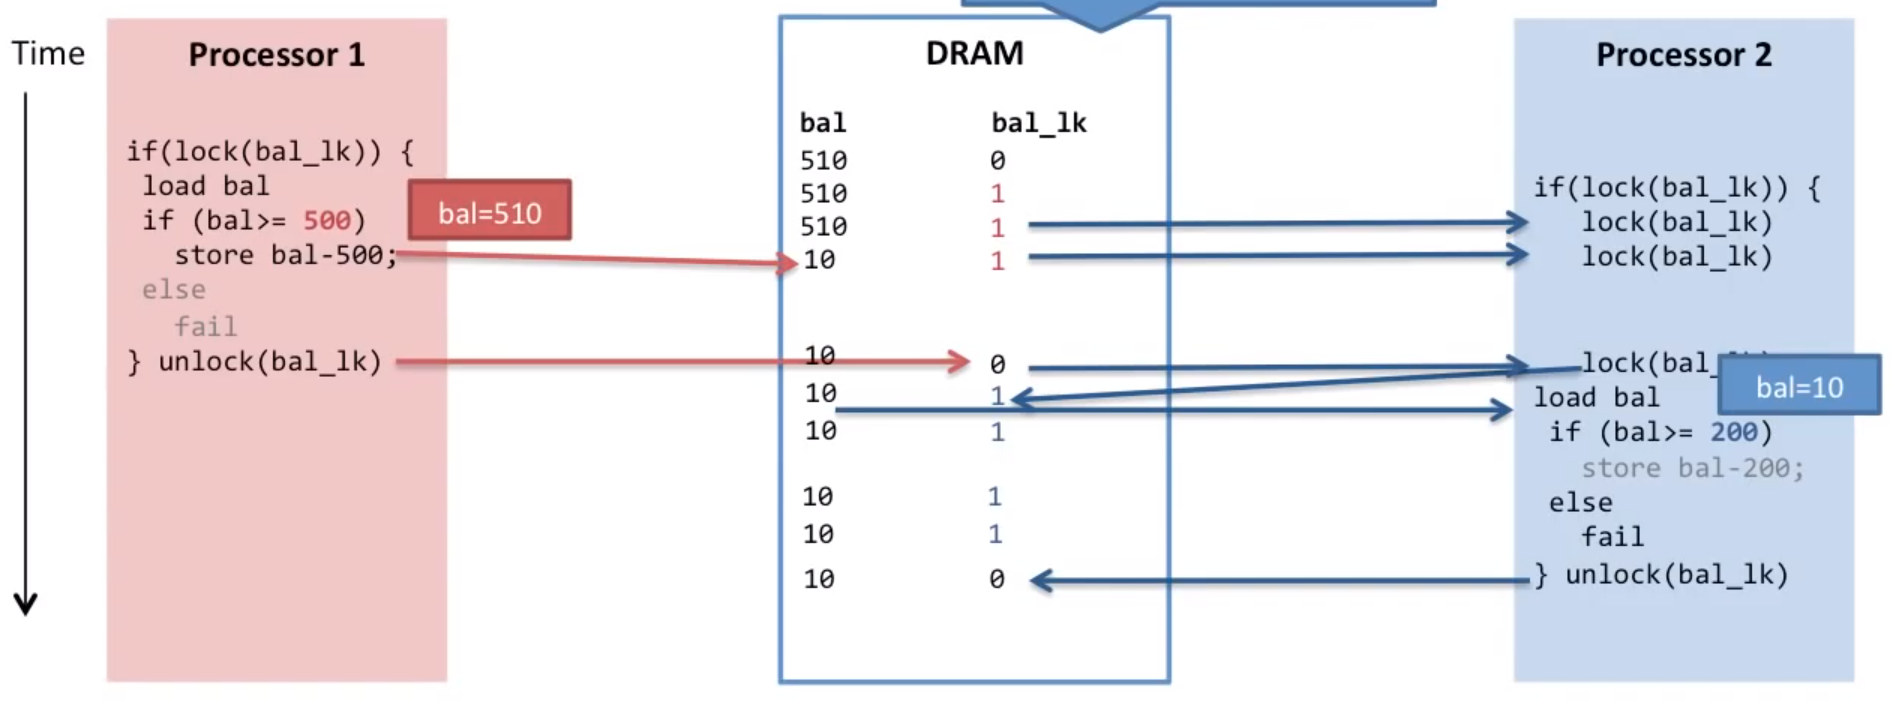
\includegraphics[width=16cm, height=7cm]{image/locks.png}
    \caption{locks}
\end{figure}


\subsection{Cache coherency}
\begin{itemize}
\item  How we use caches to save memory
\item  Locks: if the data has been accesed. (not a garanty of protection)
\item  Snooping: Look what the other processors are storing in there private cache   
\end{itemize}
  

\textbf{snooping}
\begin{figure}[h]
    \vspace{10mm}
    \centering
    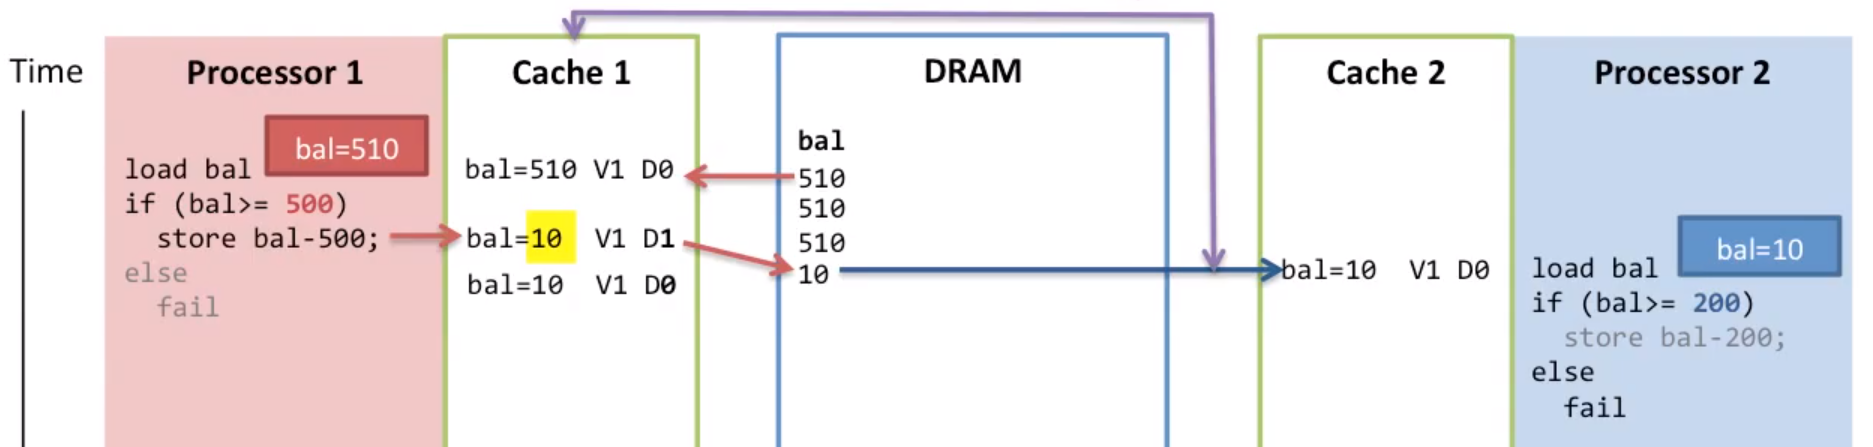
\includegraphics[width=16cm, height=5cm]{image/snooping.png}
    \caption{locks}
\end{figure}

\subsection{ILP}
\begin{itemize}
\item  Instruction level parallalism (ILP)
\item  better to have out-of-oder exicution sice we can find independent instruciions
\item  We use Dual-issue pipline so we can have one for memory instructions and
  one for non memory instruction
\item  It mrakes ISA promis with inorder exicution
\item  Issue with data hazards, more komplexity
\end{itemize}


\textbf{dual issue pipline}
\begin{figure}[h]
    \vspace{10mm}
    \centering
    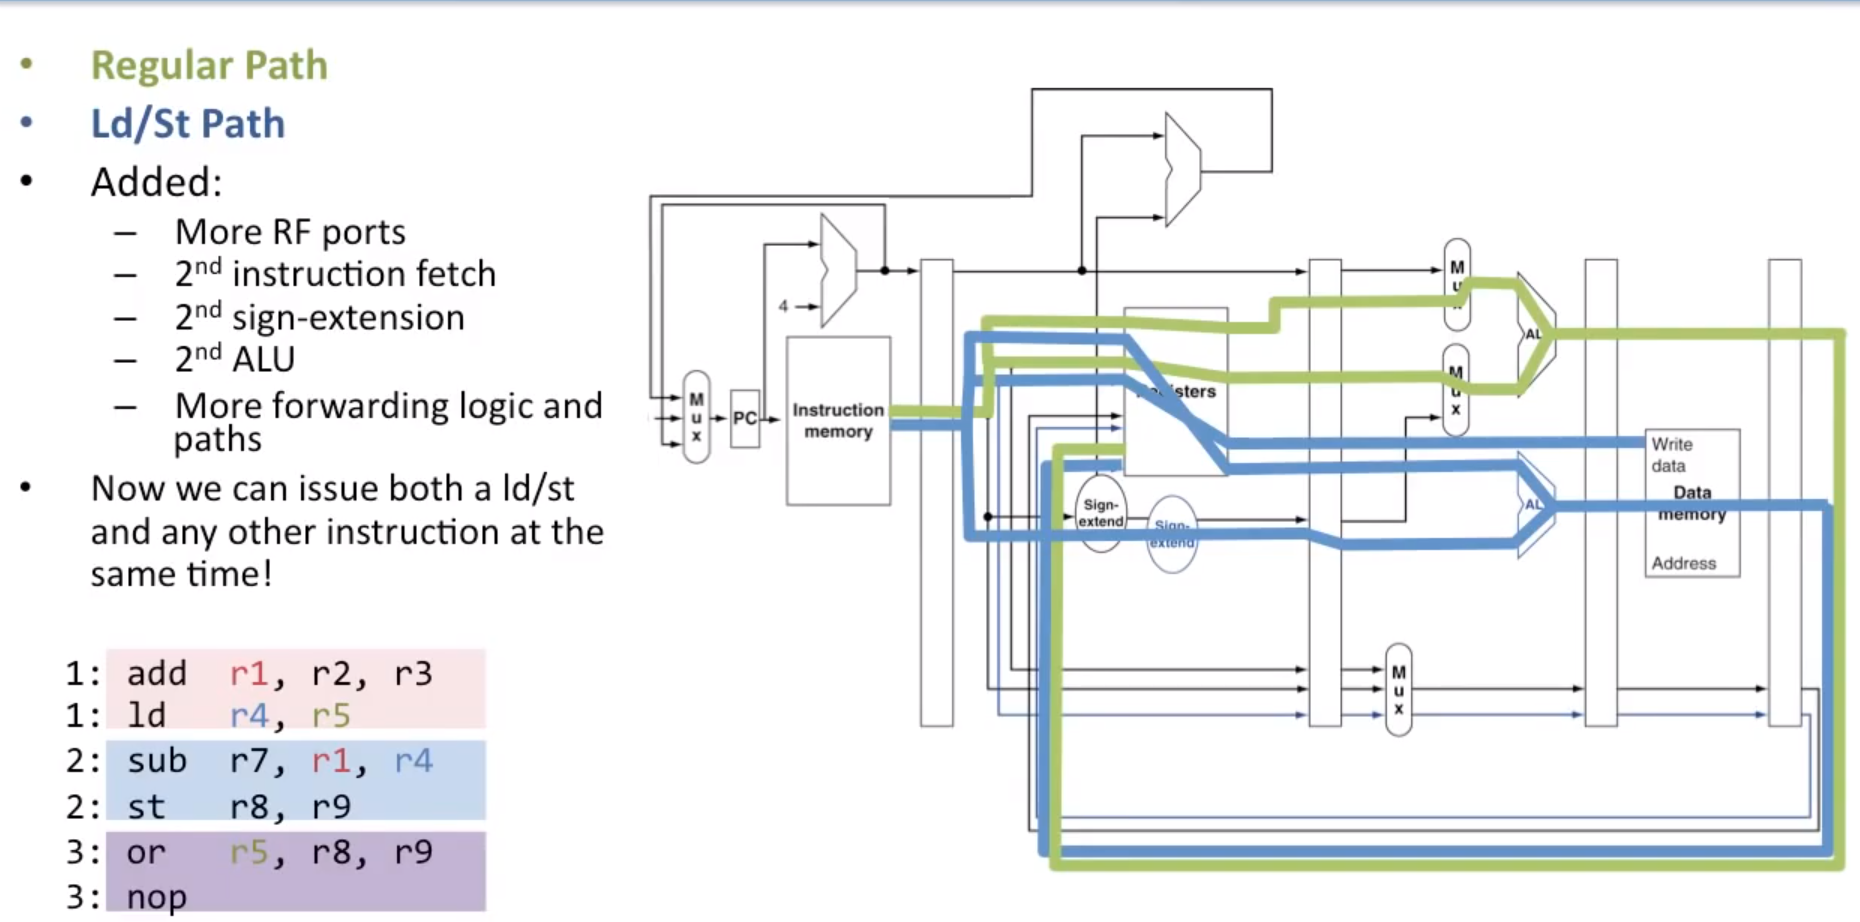
\includegraphics[width=16cm, height=7cm]{image/dual-issue-pipline.png}
    \caption{dual-issue-pipline}
\end{figure}

\textbf{Simulataneos Multithreading (SMT)}
\begin{itemize}
\item  Treads: each proscess has it own thread se it can be more easaly run in parralel
\item  SMT: allowes threads when stalled swith to another thread an run it instead  
\end{itemize}
